\chapter{remlreg objects}\normalsize
\label{remlreg} \index{remlreg object}

{\em Authors: Andreas Brezger, Thomas Kneib and Stefan Lang} \\
{\em email:
\href{mailto:andib@stat.uni-muenchen.de}{andib@stat.uni-muenchen.de},
\href{mailto:kneib@stat.uni-muenchen.de}{kneib@stat.uni-muenchen.de},
and
\href{mailto:lang@stat.uni-muenchen.de}{lang@stat.uni-muenchen.de}} \\
\vspace{0.3cm}

{\em Remlreg objects} are used to fit generalized linear models
with a {\em structured additive predictor (STAR)}, see Fahrmeir,
Kneib and Lang (2004). Inference is based on mixed model
representations of the regression models and may be seen as
empirical Bayes / posterior mode estimation. The methodological
background is provided in considerable detail in \autoref{star}.
More details on models for univariate responses can be found in
Fahrmeir, Kneib and Lang (2004), Kneib and Fahrmeir (2004a) deals
with models for multicategorical responses. A description of
models for continuous time survival analysis based on the Cox
model can be found in Kneib and Fahrmeir (2004b) Good
introductions into generalized linear models are the monographs of
Fahrmeir and Tutz (2001) and McCullagh and Nelder (1989).
Introductions to semi- and nonparametric models are given in Green
and Silverman (1994), Hastie and Tibshirani (1990), Hastie and
Tibshirani (1993) and Hastie, Tibshirani and Friedman (2001).

First steps with {\em remlreg objects} can be done with the
tutorial like example in \autoref{remlregexamples}.

\section{Method regress}
\label{remlregregress}

\subsection{Syntax}
\label{remlregregresssyntax}

 #># {\em objectname}.#regress# {\em model} [#weight# {\em weightvar}] [#if# {\em expression}] [{\em , options}] #using# {\em dataset}

Method #regress# estimates the regression model specified in {\em
model} using the data specified in {\em dataset}. {\em dataset}
must be the name of a {\em dataset object} created before. The
details of correct models are covered in
\autoref{remlregmodelsyntax}. The distribution of the response
variable can be either Gaussian, binomial, multinomial, Poisson or
gamma, see also \autoref{remlregfamilyopt} for an overview about
the models supported by {\em remlreg objects}. The response
distribution is specified using option #family#, see
\autoref{remlregfamilysyntax} below. The default is
#family=binomial# with a logit link. An #if# statement may be
specified to analyze only a part of the data set, i.e. the
observations where {\em expression} is true.

\subsubsection{Optional weight variable }
\label{remlregweightspecification}

An optional weight variable {\em weightvar} may be specified to
estimate weighted regression models. For Gaussian responses {\em
BayesX} assumes that $y_i|\eta_i,\sigma^2 \sim
N(\eta_i,\sigma^2/weightvar_i)$. Thus, for grouped Gaussian
responses the weights must be the number of observations in the
groups if the $y_i$'s are the average of individual responses. If
the $y_i$'s are the sum of responses in every group, the weights
must be the reciprocal of the number of observations in the
groups. Of course, estimation of usual weighted regression models
if the errors are heteroscedastic is also possible. In this case
the weights should be proportional to the reciprocal of the
heteroscedastic variances. If the response distribution is
binomial, it is assumed that the values of the weight variable
correspond to the number of replications and that the values of
the response variable correspond to the number of successes. If
weight is omitted, {\em BayesX} assumes that the number of
replications is one, i.e. the values of the response must be
either zero or one. For grouped Poisson data the weights must be
the number of observations in a group and the $y_i$'s are assumed
to be the average of individual responses. Weights are not allowed
for models with multicategorical response.

\subsubsection{Syntax of possible model terms}
\label{remlregmodelsyntax}

The general syntax of models for {\em remlreg objects} is:

$depvar = term_1 + term_2 + \cdots + term_r$

{\em depvar} specifies the dependent variable in the model and
$term_1$,\dots,$term_r$ define in which way the covariates
influence the dependent variable. The different terms must be
separated by '+' signs. A constant intercept is automatically
included in the models and must not be specified by the user. This
section reviews all possible model terms that are supported in the
current version of {\em remlreg objects} and provides some
specific examples. Note that all described terms may be combined
in arbitrary order. An overview about the capabilities of {\em
remlreg objects} is given in \autoref{remlregterms}.
\autoref{remlreginteractions} shows how interactions between
covariates are specified. Full details about all available options
are given in \autoref{remlreglocaloptions}.

Throughout this section Y denotes the dependent variable.

\begin{table}[ht] \footnotesize
\begin{center}
\begin{tabular}{|p{2.8cm}|p{3.6cm}|p{7.1cm}|}
\hline
{\bf Type} & {\bf Syntax example} & {\bf Description} \\
\hline \hline
offset & #offs(offset)#  & Variable #offs# is an offset term. \\
\hline
linear effect & #W1#  & Linear effect for #W1#. \\
\hline
first or second order random walk &   #X1(rw1)#  \newline  #X1(rw2)#  & Nonlinear effect of #X1#. \\
\hline
P-spline &  #X1(psplinerw1)#   \newline  #X1(psplinerw2)#  & Nonlinear effect of #X1#.  \\
\hline
seasonal prior & #time(season,period=12)# & Varying seasonal effect of #time# with period 12. \\
\hline Markov random \newline field &  #region(spatial,map=m)#  &
Spatial effect of #region# where #region# indicates the region an
observation pertains to. The boundary information and the
neighborhood structure is stored in the {\em map object}
#m#. \\
\hline Two dimensional \newline P-spline &
#region(geospline,map=m)# & Spatial effect of #region#. Estimates
a two dimensional P-spline
based on the centroids of the regions. The centroids are stored in the {\em map object} #m#. \\
 \hline
 Stationary Gaussian random field & #region(geokriging)# & Spatial effect of #region#. Estimates
a stationary Gaussian random field
based on the centroids of the regions. The centroids are stored in the {\em map object} #m#. \\
\hline
 random intercept &  #grvar(random)# & I.i.d.~(random) Gaussian effect of the group indicator #grvar#,
 e.g.~#grvar# may be an individuum indicator when analyzing longitudinal data.  \\
\hline
 baseline in Cox models & #time(baseline)# & Nonlinear shape
of the baseline effect $\lambda_0(time)$ of a Cox model. $\log(\lambda_0(time))$ is modelled by a P-spline with second order penalty. \\
 \hline
\end{tabular}
{\em \caption {\label{remlregterms} Overview over different model
terms for remlreg objects.}}
\end{center}
\end{table}


\begin{table}[ht] \footnotesize
\begin{center}
\begin{tabular}{|p{3.5cm}|p{3.8cm}|p{5.9cm}|}
\hline
{\bf Type of interaction} & {\bf Syntax example} & {\bf Description} \\
 \hline
\hline Varying coefficient term & #X1*X2(rw1)# \newline
#X1*X2(rw2)#
\newline
 #X1*X2(psplinerw1) #
 \newline  #X1*X2(psplinerw2)# \newline #X1*time(season)#
 & Effect of #X1# varies smoothly over the range of the continuous covariate #X2# or #time#, respectively. \\
\hline random slope & #X1*grvar(random)#  &  The regression
coefficient of #X1# varies with respect
to the unit- or cluster index variable #grvar#. \\
\hline Geographically weighted \newline regression &
#X1*region(spatial,map=m)#  & Effect of #X1# varies
geographically.
Covariate #region# indicates the region an observation pertains to. \\
\hline Two dimensional \newline surface &  #X1*X2(pspline2dimrw1)#
 & Two dimensional surface for the continuous
covariates #X1# and #X2#. \\
 \hline
 Stationary Gaussian random field &  #X1*X2(kriging)# & Stationary Gaussian random field for coordinates #X1# and #X2#. \\
 \hline
 Time-varying effect in Cox Models & #X1*time(baseline)# &
 Nonlinear, time-varying effect of #X1#.\\
 \hline
\end{tabular}
\caption {\label{remlreginteractions} \em Possible interaction
terms for remlreg objects.}
\end{center}
\end{table}

{\bf Offset}
\medskip

\begin{itemize}
\item[] {\em Description}: Adds an offset term to the predictor.
\item[] {\em Predictor}: $\eta =  \cdots + offs + \cdots$
\item[] {\em Syntax}: #offs(offset)#
\item[] {\em Example}:

For example, the following model statement can be used to estimate
a poisson model with #offs# as offset term and #W1# and #W2# as
fixed effects (if #family=poisson# is specified in addition):

\texttt{Y = offs(offset) + W1 + W2}
\end{itemize}

{\bf Fixed effects}
\medskip

\begin{itemize}
\item[] {\em Description}: Incorporates covariate #W1# as a fixed effect into the model.
\item[] {\em Predictor}: $\eta =  \cdots + \gamma_1 W1 + \cdots$
\item[] {\em Syntax}: #W1#
\item[] {\em Example}:

The following model statement causes #regress# to estimate a model
with $q$ fixed (linear) effects:

\texttt{Y = W1 + W2 + $\cdots$ + Wq}
\end{itemize}


{\bf Nonlinear effects of metrical covariates and time scales}
\medskip

{\em First or second order random walk}

\begin{itemize}
\item[] {\em Description}: Defines a first or second order random walk prior for the effect of #X1#.
\item[] {\em Predictor}: $\eta = \cdots + f_1(X1) + \cdots $
\item[] {\em Syntax}:

#X1(rw1#[, {\em options}]#)#

#X1(rw2#[, {\em options}]#)#
\item[] {\em Example}:

Suppose we have a continuous covariate #X1#, whose effect is
assumed to be nonlinear. The following model statement defines a
second order random walk prior for $f_1$:

#Y = X1(rw2)#

Here, the expression #X1(rw2)# indicates, that the effect of #X1#
should be incorporated nonparametrically into the model using a
second order random walk prior. A first order random walk is
specified in the model statement by modifying #rw2# to #rw1# which
yields the term #X1(rw1)#.
\end{itemize}

\vspace{0.5cm}

{\em P-spline with first or second order random walk penalty}

\begin{itemize}
\item[] {\em Description}: Defines a P-spline with a first or second order random walk penalty for
the parameters of the spline.
\item[] {\em Predictor}: $\eta =  \cdots + f_1(X1) + \cdots$
\item[] {\em Syntax}:

#X1(psplinerw1#[, {\em options}]#)#

#X1(psplinerw2#[, {\em options}]#)#
\item[] {\em Example}:

For example, a P-spline with second order random walk penalty is
obtained using the following model statement:

#Y = X1(psplinerw2)#

By default, the degree of the spline is 3 and the number of inner
knots is 20. The following model term defines a quadratic P-spline
with 30 knots:

#Y = X1(psplinerw2,degree=2,nrknots=30)#
\end{itemize}

{\em Seasonal component for time scales}

\begin{itemize}
\item[] {\em Description}: Defines a seasonal effect of #time#.
\item[] {\em Predictor}: $\eta =  \cdots + f_{season}(time) + \cdots $
\item[] {\em Syntax}:

#time(season#[, {\em options}]#)#
\item[] {\em Example}:

A seasonal component for a time scale #time# is specified for
example by

#Y = time(season,period=12)#.

Here, the second argument specifies the period of the seasonal
effect. In the example above the period is 12, corresponding to
monthly data.
\end{itemize}

{\bf Nonlinear baseline effect in Cox models}
\medskip

{\em P-spline with second order random walk penalty}

\begin{itemize}
\item[] {\em Description}: Defines a P-spline with second order
random walk penalty for the parameters of the spline for the
log-baseline effect $\log(\lambda_0$(#time#)). \item[] {\em
Predictor}: $\eta = \log(\lambda_0(time)) + \cdots$ \item[] {\em
Syntax}:

#time(baseline#[, {\em options}]#) # \item[] {\em Example}:

Suppose continuous-time survival data (#time#, #delta#) together
with additional covariates (#W1#,#X1#) are given, where #time#
denotes the vector of observed duration times, #delta# is the
vector of corresponding indicators of non-censoring, #W1# is a
discrete covariate and #X1# a continuous one. The following Cox
model with hazard rate $\lambda$ and log-baseline effect
$\log(\lambda_0$(#time#))
\begin{eqnarray*}
 \lambda(time) & = & \lambda_0(time)\exp (\gamma_0 + \gamma_1 W1 + f(X1))\\
 & = & \exp\left(\log(\lambda_0(time)) + \gamma_0 + \gamma_1 W1 + f(X1)\right)
\end{eqnarray*}
is estimated by the model statement

#delta = time(baseline) + W1 + X1(psplinerw2)#

\end{itemize}

{\bf Spatial Covariates}
\medskip

{\em Markov random field}

\begin{itemize}
\item[] {\em Description}:

Defines a Markov random field prior for the spatial covariate
#region#. {\em Remlreg objects} allow an appropriate incorporation
of spatial covariates using one of the Markov random field priors
(\ref{adjacency}) or (\ref{intrinsic}) with geographical
information stored in the {\em map object} specified through the option
#map#.
\item[] {\em Predictor}: $\eta = \cdots + f_{spat}(region) + \cdots$
\item[] {\em Syntax}:

#region(spatial,map=#{\em characterstring}[, {\em options}]#)#
\item[] {\em Example}:

The specification of a Markov random field prior for spatial data
has #map# as a required argument which must be the name of a {\em
map object} (see \autoref{map}) that contains all necessary
spatial information about the geographical map, i.e.~the neighbors
of each region and the weights associated with the neighbors. For
example the statement

#Y = region(spatial,map=germany)#

defines a Markov random field prior for #region# where the
geographical information is stored in the {\em map object} #germany#. An
error will be raised if #germany# is not existing.
\end{itemize}

\newpage

{\em 2 dimensional P-spline with first order random walk penalty}

\begin{itemize}
\item[] {\em Description}:

Defines a 2 dimensional P-spline for the spatial covariate
#region# based on the tensor product of 1 dimensional P-splines
with a 2 dimensional first order random walk penalty for the
parameters of the spline. Estimation is based on the coordinates
of the centroids of the regions an observation pertains to. The
centroids are computed using the geographical information stored
in the {\em map object} specified through the option #map#.
\item[] {\em Predictor}: $\eta= \cdots + f(centroids) + \cdots$
\item[] {\em Syntax}:

#region(geospline,map=#{\em characterstring}[, {\em options}]#)#
\item[] {\em Example}:

The specification of a 2 dimensional P-spline  (#geospline#) for
spatial data has #map# as a required argument which must be the
name of a {\em map object} (see \autoref{map}) that contains all
necessary spatial information about the geographical map, i.e.~the
neighbors of each region and the weights associated with the
neighbors. The model term

#Y = region(geospline,map=germany)#

specifies a tensor product cubic P-spline with first order random
walk penalty where the geographical information is stored in the
{\em map object} #germany#.
\end{itemize}

\vspace{0.5cm}

{\bf Unordered group indicators}
\medskip

{\em Unit- or cluster specific unstructured effect}

\begin{itemize}
\item[] {\em Description}: Defines an unstructured (uncorrelated) random effect with respect
to grouping variable #grvar#.
\item[] {\em Predictor}: $\eta = \cdots + f(grvar) + \cdots$
\item[] {\em Syntax}:

#grvar(random#[, {\em options}]#)#
\item[] {\em Example}:

Method regress supports Gaussian i.i.d.~random effects to cope
with unobserved heterogeneity among units or clusters of
observations. Suppose the analyzed data set contains a group
indicator #grvar# that gives information about the individual or
cluster a particular observation belongs to. Then an individual
specific uncorrelated random effect is incorporated through the
term

#Y = grvar(random)#

The inclusion of more than one random effect term in the model is
possible, allowing the estimation of multilevel models. However,
we have only limited experience with multilevel models so that it
is not clear how well these models can be estimated using {\em
remlreg objects}.
\end{itemize}

\newpage

{\bf Varying coefficients with metrical covariates as effect
modifier} \medskip

{\em First or second order random walk}

\begin{itemize}
\item[] {\em Description}:

Defines a varying coefficient term, where the effect of #X1# varies
smoothly over the range of #X2#. Covariate #X2# is the effect
modifier. The smoothness prior for $f$ is a first or second order
random walk.
\item[] {\em Predictor}: $\eta= \cdots + f(X2)X1 + \cdots$
\item[] {\em Syntax}:

#X1*X2(rw1#[, {\em options}]#)#

#X1*X2(rw2#[, {\em options}]#)#
\item[] {\em Example}:

For example, a varying coefficient term with a second order random
walk smoothness prior is defined as follows:

#Y = X1*X2(rw2)#
\end{itemize}


{\em P-spline with first or second order random walk penalty}
\begin{itemize}
\item[] {\em Description}:

Defines a varying coefficient term, where the effect of #X1# varies
smoothly over the range of #X2#. Covariate #X2# is the effect
modifier. The smoothness prior for $f$ is a P-spline with first or
second order random walk penalty.
\item[] {\em Predictor}: $\eta= \cdots + f(X2)X1 + \cdots$
\item[] {\em Syntax}:

#X1*X2(psplinerw1#[, {\em options}]#)#

#X1*X2(psplinerw2#[, {\em options}]#)#
\item[] {\em Example}:

For example, a varying coefficient term with a second order random
walk smoothness prior is defined as follows:

#Y = X1*X2(psplinerw2)#

\end{itemize}

{\em Seasonal prior}
\begin{itemize}
\item[] {\em Description}:

Defines a varying coefficients term where the effect of #X1# varies
over the range of the effect modifier #time#. For #time# the
seasonal prior (\ref{seasonal}) is used.
\item[] {\em Predictor}: $\eta= \cdots + f_{season}(time)X1 + \cdots $
\item[] {\em Syntax}:

#X1*time(season#[, {\em options}]#)#
\item[] {\em Example}:

The inclusion of a varying coefficients term with a seasonal prior
may be meaningful if we expect a different seasonal effect with
respect to grouping variable #X1#. In this case we can include
additional seasonal effects for each category of #X1# by

#Y = X1*time(season)#

\end{itemize}

{\bf Time-varying effects in Cox models}
\medskip

{\em P-spline with second order random walk penalty}

\begin{itemize}
\item[] {\em Description}: Defines a varying coefficients term
where the effect of #X1# varies over the range of the effect
modifier #time#, i.e. variable #X1# has time-varying effect. The
smoothness prior for $f($#time#$)$ is a P-spline with second order
random walk penalty.

 \item[] {\em Predictor}: $\eta = \log(\lambda_0(time)) +
f(time)X1 \cdots$ \item[] {\em Syntax}:

 #X1*time(baseline#[, {\em options}]#) #
 \item[] {\em Example}:

Suppose continuous-time survival data (#time#, #delta#) together
with an additional covariate #X1# are given, where #time# denotes
the vector of observed duration times, #delta# is the vector of
corresponding indicators of non-censoring. The following Cox model
with hazard rate $\lambda$
\begin{eqnarray*}
 \lambda(time) & = & \lambda_0(time)\exp(\gamma_0 + f(time)X1)\\
 & = & \exp\left(\log(\lambda_0(time)) + \gamma_0 + f(time)X1\right)
\end{eqnarray*}
is estimated by the model statement

#delta = time(baseline) + X1*time(baseline)#

\end{itemize}


{\bf Varying coefficients with spatial covariates as effect
modifiers} \medskip

{\em Markov random field}

\begin{itemize}
\item[] {\em Description}:

Defines a varying coefficient term where the effect of #X1# varies
smoothly over the range of the spatial covariate #region#. A
Markov random field is estimated for $f_{spat}$. The geographical
information is stored in the {\em map object} specified through the
option #map#.
\item[] {\em Predictor}: $\eta = \cdots + f_{spat}(region)X1 + \cdots$
\item[] {\em Syntax}:

#X1*region(spatial,map=#{\it characterstring} #[,# {\it options}#])#
\item[] {\em Example}:

For example the statement

#Y = X1*region(spatial,map=germany)#

defines a varying coefficient term with the spatial covariate
#region# as the effect modifier and the spatial smoothness prior
(\ref{adjacency}), or the more general prior (\ref{intrinsic})
depending on the weight definition in the {\em map object} #germany#.
\end{itemize}

{\bf Varying coefficients with unordered group indicators as
effect modifiers (random slopes)}
\medskip

{\em Unit- or cluster specific unstructured effect}
\begin{itemize}
\item[] {\em Description}:

Defines a varying coefficient term where the effect of #X1# varies
over the range of the group indicator #grvar#. Models of this type
are usually referred to as models with random slopes. A Gaussian
i.i.d.~random effect with respect to grouping variable #grvar# is
assumed for $f$.
\item[] {\em Predictor}: $\eta = \cdots + f(grvar)X1 + \cdots$
\item[] {\em Syntax}:

#X1*grvar(random#[, {\em options}]#)#
\item[] {\em Example}:

For example, a random slope is specified as follows:

#Y = X1*grvar(random)#

Note, that in contrast to {\em bayesreg objects} no main effects
are included automatically. If main effects should be included in
the model, they have to be specified as additional fixed effects.
The syntax for obtaining the predictor

{\em Predictor}: $\eta = \cdots + \gamma X1 + f(grvar)X1 + \cdots$

would be

#X1 + X1*grvar(random#[, {\em options}]#)#

\end{itemize}


{\bf Surface estimators}
\medskip

{\em 2 dimensional P-spline with first order random walk penalty}
\begin{itemize}
\item[] {\em Description}:

Defines a 2 dimensional P-spline based on the tensor product of 1
dimensional P-splines with a 2 dimensional first order random walk
penalty for the parameters of the spline.
\item[] {\em Predictor}: $\eta= \cdots + f(X1,X2) + \cdots$
\item[] {\em Syntax}:

#X1*X2(pspline2dimrw1#[, {\em options}]#)#
\item[] {\em Example}:

The model term

#Y = X1*X2(pspline2dimrw1)#

specifies a tensor product cubic P-spline with first order random
walk penalty.

In many applications it is favorable to additionally incorporate
the 1 dimensional main effects of #X1# and #X2# into the models. In
this case the 2 dimensional surface can be seen as the deviation
from the main effects. Note, that in contrast to {\em bayesreg
objects} the number of inner knots and the degree of the spline
may be different for the main effects and for the interaction. For
example, a model with 20 inner knots for the main effects and 10
inner knots for the 2 dimensional P-Spline is estimated by

 #Y = X1(psplinerw2,nrknots=20) + X2(psplinerw2,nrknots=20)#\\
 #    + X1*X2(pspline2dimrw1,nrknots=10)#
\end{itemize}

{\em Stationary Gaussian random field}
\begin{itemize}
\item[] {\em Description}:

Defines that the parameters of the locations follow a stationary
Gaussian random field. Depending on the chosen options, locations
are given either by the distinct pairs of #X1# and #X2# or by a
subset of these pairs, which we will also refer to as knots. Note
that, although stationary Gaussian random fields can be used to
estimate surfaces depending on arbitrary variables #X1# and #X2#,
they are defined based on {\em isotropic} correlation functions.
This means that correlations between sites that have the same
distance also have the same correlation, regardless of direction
and the sites location. Therefore, if Gaussian random fields shall
be used to estimate interactions between variables that do not
represent longitude and latitude, these variables have to be
standardized appropriately.

\item[] {\em Predictor}: $\eta= \cdots + f(X1,X2) + \cdots$
\item[] {\em Syntax}:

#X1*X2(kriging#[, {\em options}]#)# \item[] {\em Example}:

The model term

#Y = X1*X2(kriging,nrknots=100)#

specifies a stationary Gaussian random field for the effect of
#X1# and #X2# with 100 knots, which are computed based on the
space filling algorithm described in \autoref{interactions}. If
all distinct pairs of #X1# and #X2# shall be used as knots, we
have to specify

#Y = X1*X2(kriging,full)#

Note, that the knots computed by the space filling algorithm are
stored in the outfile directory of the {\em remlreg object}. These
knots can be read into a {\em dataset object} which may be passed
in the call of method #regress# if we want to use the same knots
as in previous calls:

 #dataset kn#\\
 #kn.infile using #{\em knotfile}\\
 #Y = X1*X2(kriging,knotdata=kn)#

To determine the actual number of knots, the options are
interpreted in a specific sequence. If option #full# is specified,
both #nrknots# and #knotdata# are ignored. Similarly, #nrknots# is
ignored if #knotdata# is specified.

\end{itemize}

\subsubsection{Description of additional options for terms of {\em remlreg objects}}
\label{remlreglocaloptions}

All arguments described in this section are optional and may be
omitted. Generally, options are specified by adding the option
name to the specification of the model term type in the
parentheses, separated by comma. Note that all options may be
specified in arbitrary order. \autoref{remlregoptions} provides
explanations and the default values of all possible options. In
\autoref{remlregtermsoptions} all reasonable combinations of model
terms and options can be found.

\begin{table}[ht] \footnotesize \centering
\begin{tabular}{|p{0.1\linewidth}|p{0.6\linewidth}|p{0.2\linewidth}|}
 \hline
 optionname & description & default\\
 \hline\hline
 #lambdastart# & Provides a starting value for the smoothing parameter $\lambda$. & #lambdastart=10# \\
 \hline
 #degree# & Specifies the degree of the B-spline basis functions. & #degree=3# \\
 \hline
 #nrknots# & Specifies the number of inner knots for a P-spline term or the number of knots for a kriging term. & #nrknots=20# (P-splines)\newline #nrknots=100# (kriging)  \\
 \hline
 #knotdata# & {\em Dataset object} containing the knots to be used
 with the kriging term & no default.\\
 \hline
 #full# & Specifies that all distinct locations should be used as
 knots with the kriging term. & -\\
 \hline
 #nu# & The smoothness parameter $\nu$ of the Mat\`{e}rn correlation function. & #nu=1.5# \\
 \hline
 #maxdist# & Specifies the value $c$ that is used to determine the scale parameter $\rho$ of the Mat\`{e}rn correlation function. Compare \autoref{interactions}. & default depends on #nu#\\
 \hline
 #p# & Defines the parameter $p$ used in the coverage criterion of the space filling algorithm. & #p=-20#\\
 \hline
 #q# & Defines the parameter $q$ used in the coverage criterion of the space filling algorithm. & #q=20#\\
 \hline
 #maxsteps# & Specifies the maximum number of steps to be performed by the space filling algorithm. & #maxsteps=300#\\
 \hline
 #gridchoice# & How to choose grid points for numerical integration in Cox models. May be either '#quantiles#' or '#equidistant#'. & #gridchoice=quantiles# \\
 \hline
 #tgrid# & Number of equidistant time points to be used for numerical integration in Cox models. Only meaningful if #gridchoice=equidistant#. & #tgrid=100#\\
 \hline
 #nrquantiles# & Number of quantiles that are used to define the grid points for numerical integration in Cox models. First a grid of #nrquantiles# quantiles is computed, then the grid for integration is defined by #nrbetween# equidistant points between each quantile. Only meaningful if #gridchoice=quantiles#. & #nrquantiles=50#\\
 \hline
 #nrbetween# & Number of points between quantiles that are used to define the grid points for numerical integration in Cox models. First a grid of #nrquantiles# quantiles is computed, then the grid for integration is defined by #nrbetween# equidistant points between each quantile. Only meaningful if #gridchoice=quantiles#.& #nrbetween=5#\\
 \hline
 #map# & {\em Map object} for spatial effects. & no default\\
 \hline
 #period# & The period of the seasonal effect can be specified with the option #period#. The default is #period=12# which corresponds to monthly data. & #period=12# \\
 \hline
\end{tabular}
{\em \caption{\label{remlregoptions} Optional arguments for {\em
remlreg object} terms}}
\end{table}

\begin{sidewaystable} \footnotesize
\begin{tabular}{|l||c|c|c|c|c|c|c|c|c|c|}

\hline
            & rw1/rw2       & season    & psplinerw1/psplinerw2    & spatial & random & geospline & pspline2dimrw1 & kriging  & geokriging & baseline\\
 \hline\hline
 #lambdastart#$^*$  & realvalue   & realvalue   & realvalue   & realvalue   & realvalue   & realvalue   & realvalue & realvalue  & realvalue & realvalue\\
 \hline
 #degree#       & $\times$   & $\times$   &  integer   & $\times$ & $\times$ &  integer &  integer &  $\times$ & $\times$ & integer\\
 \hline
 #nrknots#      & $\times$   & $\times$   &  integer   & $\times$ & $\times$ &  integer &  integer &  integer & $\times$ & integer\\
 \hline
 #knotdata#     & $\times$   & $\times$   &  $\times$   & $\times$ & $\times$ &  $\times$ &  $\times$ & {\em dataset object}& {\em dataset object} & $\times$\\
 \hline
 #full#     & $\times$   & $\times$   &  $\times$   & $\times$ & $\times$ &  $\times$ &  $\times$ &  $\triangle$ & $\triangle$ & $\times$\\
 \hline
 #nu#     & $\times$   & $\times$   &  $\times$   & $\times$ & $\times$ &  $\times$ &  $\times$ &  $\bullet$ &  $\bullet$ & $\times$\\
 \hline
 #maxdist#$^*$     & $\times$   & $\times$   &  $\times$   & $\times$ & $\times$ &  $\times$ &  $\times$ &  realvalue &  realvalue &  $\times$\\
 \hline
 #p#$^{**}$     & $\times$   & $\times$   &  $\times$   & $\times$ & $\times$ &  $\times$ &  $\times$ &  realvalue &  realvalue &  $\times$\\
 \hline
 #q#$^*$     & $\times$   & $\times$   &  $\times$   & $\times$ & $\times$ &  $\times$ &  $\times$ &  realvalue &  realvalue &  $\times$\\
 \hline
 #maxsteps#     & $\times$   & $\times$   &  $\times$   & $\times$ & $\times$ &  $\times$ &  $\times$ &  integer  &  integer & $\times$\\
 \hline
 #gridchoice#   & $\times$  & $\times$  & $\times$  & $\times$  & $\times$  & $\times$  & $\times$  & $\times$  & $\times$ & $\circ$\\
 \hline
 #tgrid#   & $\times$  & $\times$  & $\times$  & $\times$  & $\times$  & $\times$  & $\times$  & $\times$  & $\times$ & integer\\
 \hline
 #nrquantiles#   & $\times$  & $\times$  & $\times$  & $\times$  & $\times$  & $\times$  & $\times$  & $\times$  & $\times$ & integer\\
 \hline
 #nrbetween#   & $\times$  & $\times$  & $\times$  & $\times$  & $\times$  & $\times$  & $\times$  & $\times$  & $\times$ & integer\\
 \hline
 #period#      & $\times$   & integer     & $\times$  & $\times$      & $\times$  & $\times$ & $\times$ & $\times$  & $\times$ & $\times$\\
 \hline
 #map#      & $\times$   & $\times$     & $\times$  & {\em map object}  & $\times$  & {\em map object} & $\times$ & $\times$ & {\em map object} & $\times$ \\
 \hline \hline
 $^*$ & \multicolumn{10}{l|}{positive values only}\\
 \hline
 $^{**}$ & \multicolumn{10}{l|}{negative values only}\\
 \hline
 $\times$    & \multicolumn{10}{l|}{not available} \\
 \hline
 $\bullet$  & \multicolumn{10}{l|}{admissible values are #0.5,1.5,2.5,3.5#} \\
 \hline
 $\triangle$   & \multicolumn{10}{l|}{available as boolean option (specified without supplying a value)} \\
 \hline
 $\circ$  & \multicolumn{10}{l|}{admissible values are '#quantiles#' and '#equidistant#'} \\
 \hline
\end{tabular}
{\em\centering \caption{\label{remlregtermsoptions} Terms and
options for remlreg objects}}
\end{sidewaystable}

\subsubsection{Specifying the response distribution}
\label{remlregfamilysyntax}

The current version of {\em BayesX} supports the most common
univariate distributions of the response for the use with {\em
remlreg objects}. These are Gaussian, binomial (with logit or
probit link), Poisson and gamma. An overview over the supported
models is given in \autoref{remlregfamilyopt}. In {\em BayesX} the
distribution of the response is specified by adding the additional
option #family# to the options list of the regress command. For
instance, #family=gaussian# defines the responses to be Gaussian.
In the following we give detailed instructions on how to specify
the different models:

\begin{table}[ht]
\begin{center}
\begin{tabular} {|l|l|p{2.7cm}|l|}
 \hline
 value of #family# & response distribution & link & options\\
 \hline
 \hline
 #family=gaussian#            & Gaussian              & identity & \\
 \hline
 #family=binomial#            & binomial              & logit & \\
 #family=binomialprobit#      & binomial              & probit & \\
 #family=binomialcomploglog#      & binomial              & complementary log-log & \\
 \hline
 #family=multinomial#         & unordered multinomial & logit & #reference#\\
 \hline
 #family=cumprobit#           & cumulative multinomial   & probit & \\
 #family=cumlogit#            & cumulative multinomial   & logit & \\
 \hline
 #family=poisson#             & Poisson               & log-link & \\
 \hline
 #family=gamma#               & gamma                 & log-link & \\
 \hline
 #family=cox#                 & continuous-time survival data & & \\
 \hline
\end{tabular}
{\em \caption {\label{remlregfamilyopt} Summary of supported
response distributions.}}
\end{center}
\end{table}

{\bf Gaussian responses}

For Gaussian responses {\em BayesX} assumes $y_i | \eta_i,\sigma^2
\sim N(\eta_i,\sigma^2/weightvar_i)$ or equivalently in matrix
notation $y | \eta, \sigma^2 \sim N(\eta,\sigma^2C^{-1})$. Here
$C^{-1}=diag(weightvar_1,\dots,weightvar_n)$ is a known covariance
matrix. Gaussian response is specified by adding

#family=gaussian#

to the options list.

An optional weight variable {\em weightvar} may be specified to
estimate weighted regression models, see
\autoref{remlregregresssyntax} for the syntax. For grouped
Gaussian responses the weights must be the number of observations
in the groups if the $y_i$'s are the average of individual
responses. If the $y_i$'s are the sum of responses in every group,
the weights must be the reciprocal of the number of observations
in the groups. Of course, estimation of usual weighted regression
models if the errors are heteroscedastic is also possible. In this
case the weights should be proportional to the reciprocal of the
heteroscedastic variances. If a weight variable is not specified,
{\em BayesX} assumes $weightvar_i = 1$, $i=1,\dots,n$.

{\bf Binomial logit, probit and complementary log-log models}

A binomial logit model is specified by adding the option

#family=binomial#

a probit model by adding

#family=binomialprobit#

and a complementary log-log model by adding

#family=binomialcomploglog#

to the option list.

A weight variable may be additionally specified, see
\autoref{remlregregresssyntax} for the syntax. {\em BayesX}
assumes that the weight variable corresponds to the number of
replications and the response variable to the number of successes.
If the weight variable is omitted, {\em BayesX} assumes that the
number of replications is one, i.e.~the values of the response
must be either zero or one.

{\bf Multinomial logit models}

So far {\em remlreg objects} support only multinomial logit
models. A multinomial logit model is specified by adding the
option

#family=multinomial#

to the options list.

Usually a second option must be added to the options list to
define the reference category. This is achieved by specifying the
#reference# option. Suppose that the response variable has three
categories 1,2 and 3. To define, for instance, the reference
category to be 2, simply add

#reference=2 #

to the options list. If this option is omitted, the {\em smallest}
number will be used as the reference category.

{\bf Cumulative logit and probit models}

A cumulative logit model is specified by adding

#family=cumlogit#

to the options list, a cumulative probit model by adding

#family=cumprobit#

to the options list. The reference category will always be the
largest value of the response.

Note, that in contrast to {\em bayesreg objects} {\em remlreg
objects} can deal with an arbitrary number of ordered categories.
However, for more than 5 categories estimation will become rather
computer intensive and time demanding.

{\bf Poisson regression}

A Poisson regression is specified by adding

#family=poisson#

to the options list.

A weight variable may be additionally specified, see
\autoref{remlregregresssyntax} for the syntax. For grouped Poisson
data the weights must be the number of observations in a group and
the responses are assumed to be the average of individual
responses.

{\bf Gamma distributed responses}

In the literature, the density function of the gamma distribution
is parameterized in various ways. In the context of regression
analysis the density is usually parameterized in terms of the mean
$\mu$ and the scale parameter $s$. Then, the density of a gamma
distributed random number $y$ is given by
\begin{equation}
\label{remlgammapar1} p(y) \propto y^{s-1}\exp(-\frac{s}{\mu} y)
\end{equation}
for $y > 0$. For the mean and the variance we obtain $E(y) = \mu$
and $Var(y) = \mu^2/s$. We write $y \sim G(\mu,s)$

A second parameterization is based on hyperparameters $a$ and $b$
and is usually used in the context of Bayesian hierarchical models
to specify hyperpriors for variance components. The density is
then given by
\begin{equation}
\label{remlgammapar2} p(y) \propto y^{a-1}\exp(-b y)
\end{equation}
for $y>0$. In this parameterization we obtain $E(y) = a/b$ and
$Var(y) = a/b^2$ for the mean and the variance, respectively. We
write $y \sim G(a,b)$

In {\em BayesX} gamma distributed response is defined in the first
parameterization (\ref{remlgammapar1}). For the $r$th observation
{\em BayesX} assumes  $y_r | \eta_r,\nu \sim
G(\exp(\eta_r),\nu/weightvar_r)$ where $\mu_r = \exp(\eta_r)$ is
the mean and $s=\nu/weightvar_r$ is the scale parameter. Gamma
distributed response is specified by adding

#family=gamma#

to the options list. An optional weight variable {\em weightvar}
may be specified to estimate weighted regression models. In this
case the weights should be proportional to the reciprocal of the
heteroscedastic variances, see \autoref{remlregregresssyntax} for
the syntax.

\textbf{Continuous time survival analysis}

\textit{BayesX} offers two alternatives of estimating continuous
time Cox models with semiparametric predictor $\eta$, which are
described in \autoref{continuoustime}. The first alternative is to
assume that all time-dependent values are piecewise constant,
which leads to the so called \textit{piecewise exponential model}
(p.e.m.), and the second one is to estimate the log-baseline
effect $\log(\lambda_0(t))=f_0(t)$ by a P-spline with second order
random walk penalty.

\textbf{Piecewise exponential model (p.e.m.)}

In \autoref{continuoustime} we demonstrated how continuous time
survival data has to be manipulated such that a Poisson model may
be used for estimation. Suppose now we have the modified data set
\vspace{0.5cm}\\
\begin{tabular}{c|c|c|c|c|c|c}
#y# & #indnr# & #a# & $\delta$ &  $\Delta$ &   #x1# &
#x#2\\\hline\hline
0 &  1 &   0.1 &   1  &  log(0.1) & 0  & 3\\
0  & 1   & 0.2  &  1  &  log(0.1) & 0 &  3\\
1  & 1   & 0.3  &  1  &  log(0.05)& 0  & 3\\\hline
0 &  2 &   0.1 &   0 &   log(0.1) & 1 &  5\\
0  & 2  &  0.2 &   0  &  log(0.02)& 1 &  5\\\hline
$\vdots$ & $\vdots$ & $\vdots$ & $\vdots$ & $\vdots$ & $\vdots$& $\vdots$\\
\end{tabular}
\vspace{0.5cm}\\
with indicator #y#, interval limit #a#, indicator of non-censoring
$\delta$ and offset $\Delta$ defined as in
\autoref{continuoustime}. Let #x1# be a covariate with linear
effect and #x2# a continuous one with a nonlinear effect. Then the
correct syntax for estimating a p.e.m.~with a {\em remlreg object}
named #r# is e.g.~as follows:

 #> r.regress y = a(rw1) + Delta(offset) + x1 + x2(psplinerw2), family=poisson# $\ldots$

or

 #> r.regress y = a(rw2) + Delta(offset) + x1 + x2(psplinerw2), family=poisson# $\ldots$

Note that a time-varying effect of a covariate #X# may be
estimated in the p.e.m.~by adding the term

#X*a(rw1) or X*a(rw2)#

to the model statement.

\textbf{Specifying a P-spline prior for the log-baseline}

For the estimation of a Cox model with a P-spline prior with
second order random walk penalty

#family=cox#

has to be specified in the options list. The number of knots and
degree of the P-spline prior for $f_0(t)$ may be specified in the
baseline term. The indicator of non-censoring $\delta_i$ has to be
specified as the dependent variable in the model statement. Data
augmentation and the specification of an offset term are not
required here.

In the example above with survival data

\vspace{0.5cm}

\begin{tabular}{c|c|c|c}
  #t# &   $\delta$ &  #x1# &  #x2#\\\hline\hline
0.25  &  1  &    0  &  3\\\hline 0.12  &  0  &    1  &  5\\\hline
$\vdots$ & $\vdots$ & $\vdots$ & $\vdots$ \\
\end{tabular}
\vspace{0.5cm}\\
a Cox model with a quadratic P-spline prior with 15 knots for the
log-baseline would be estimated as follows:

 #> r.regress delta = t(baseline,degree=2,nrknots=15)+ x1 + x2(psplinerw2),#\\
 #  family=cox# \ldots

Note, that we assume that a {\em remlreg object} #r# has been
created before executing the command.

\subsection{Options}
\label{remlregregressoptions}

\vspace{0.4cm}

{\bf Options for controlling the estimation process}
\label{remlest_options}

Options for controlling estimation process are listed in
alphabetical order.

\begin{itemize}
\item {\bf eps = realvalue } \\
\\Defines the termination criterion of the estimation process. If
both the relative changes in the regression coefficients and the
variance parameters are less than #eps#, the estimation process is
assumed to have converged.\\
DEFAULT: #eps = 0.00001#

\item {\bf lowerlim = realvalue } \\
Since small variances are near to the boundary of their parameter
space, the usual Fisher-scoring algorithm for their determination
has to be modified. If the fraction of the penalized part of an
effect relative to the total effect is less than #lowerlim#, the
estimation of the corresponding variance is stopped and the
estimator is defined to be the current value of the variance (see
\autoref{remlstopcrit} for details).\\
DEFAULT: #lowerlim = 0.001#

\item {\bf maxit = integer } \\
Defines the maximum number of iterations to be used in estimation.
Since the estimation process will not necessarily converge, it may
be useful to define an upper bound for the number of iterations.
Note, that {\it BayesX} produces results based on the current
values of all parameters even if no convergence could be achieved
within #maxit# iterations, but a warning message will be printed
in the {\it output window}.\\
DEFAULT: #maxit=400#

\end{itemize}

{\bf Further options} \label{remlreg further options}

\index{credible intervals} \index{credible intervals!changing the
nominal level} \index{changing the nominal level of credible
intervals}\index{remlreg object!credible intervals}
\begin{itemize}
\item \label{remlreglevel1} {\bf level1 = integer} \\
Besides the posterior mode, #regress# provides (approximate)
pointwise posterior credible intervals for every effect in the
model. By default, {\em BayesX} computes credible intervals for
nominal levels of 80\% and 95\%. The option #level1# allows to
redefine one of the nominal levels (95\%). Adding, for instance,

#level1=99 #

to the option list leads to the computation of credible intervals
for a nominal level of 99\% rather than 95\%.
\item \label{remlreglevel2} {\bf level2 = integer} \\
Besides the posterior mode, #regress# provides (approximate)
pointwise posterior credible intervals for every effect in the
model. By default, {\em BayesX} computes credible intervals for
nominal levels of 80\% and 95\%. The option #level2# allows to
redefine one of the nominal levels (95\%). Adding, for instance,

#level2=70#

to the option list leads to the computation of credible intervals
for a nominal level of 70\% rather than 80\%.
\end{itemize}

\subsection{Estimation output}

The way the estimation output is presented depends on the
estimated model. Estimation results for fixed effects are
displayed in a tabular form in the {\em output window} and/or in a
log file (if created before). Shown will be the posterior mode,
the standard deviation, p-values and an approximate 95\% credible
interval. Other credible intervals may be obtained by specifying
the #level1# option, see \autoref{remlreg further options} for
details. Additionally a file is created where estimation results
for fixed effects are replicated. The name of the file is given in
the {\em output window} and/or in a log file.

Estimation effects for nonparametric effects are presented in a
different way. Here, results are stored in external ASCII-files
whose contents can be read into any general purpose statistics
program (e.g. STATA, S-plus) to further analyze and/or visualize
the results. The structure of these files is as follows: There
will be one file for every nonparametric effect in the model. The
name of the files and the storing directory are displayed in the
{\em output window} and/or a log file. The files contain ten or
eleven columns, depending on whether the corresponding model term
is an interaction effect. The first column contains a parameter
index (starting with one), the second column (and the third column
if the estimated effect is a 2 dimensional P-spline) contain the
values of the covariate(s) whose effect is estimated. In the
following columns the estimation results are given in form of the
posterior mode, the lower boundaries of the (approximate) 95\% and
80\% credible intervals, the standard deviation and the upper
boundaries of the 80\% and 95\% credible intervals. The last two
columns contain approximations to the posterior probabilities
based on nominal levels of 95\% and 80\%. A value of 1 corresponds
to a strictly positive 95\% or 80\% credible interval and a value
of -1 to a strictly negative credible interval. A value of 0
indicates that the corresponding credible interval contains zero.
Other credible intervals and posterior probabilities may be
obtained by specifying the #level1# and/or #level2# option, see
\autoref{remlreg further options} for details. As an example
compare the following lines, which are the beginning of a file
containing the results for a nonparametric effect of a particular
covariate, x say:

\footnotesize
 intnr \,\, x \,\, pmode \,\, ci95lower \,\, ci80lower \,\, std \,\, ci80upper \,\, ci95upper \,\, pcat95 \,\, pcat80\\
 1 \,\, -2.87694 \,\, -0.307921 \,\, -0.886815 \,\, -0.686408 \,\, 0.295295 \,\, 0.070567   \,\, 0.270973 \,\, 0 \,\, 0\\
 2 \,\, -2.86203 \,\, -0.320479 \,\, -0.885375 \,\, -0.689815 \,\, 0.288154 \,\, 0.0488558  \,\, 0.244416 \,\, 0 \,\, 0\\
 3 \,\, -2.8515  \,\, -0.329367 \,\, -0.88473  \,\, -0.69247  \,\, 0.283292 \,\, 0.0337362  \,\, 0.225997 \,\, 0 \,\, 0\\
 4 \,\, -2.85066 \,\, -0.330072 \,\, -0.884692 \,\, -0.692689 \,\, 0.282913 \,\, 0.0325457  \,\, 0.224549 \,\, 0 \,\, 0\\
 5 \,\, -2.82295 \,\, -0.3535   \,\, -0.884544 \,\, -0.700703 \,\, 0.270887 \,\,-0.00629671 \,\, 0.177545 \,\, 0 \,\, -1\\
 6 \,\, -2.79856 \,\, -0.37418  \,\, -0.886192 \,\, -0.708939 \,\, 0.261178 \,\,-0.0394208  \,\, 0.137832 \,\, 0 \,\, -1\\
 7 \,\, -2.79492 \,\, -0.377272 \,\, -0.886579 \,\, -0.710263 \,\, 0.259798 \,\,-0.0442813  \,\, 0.132035 \,\, 0 \,\, -1\\
 8 \,\, -2.79195 \,\, -0.379788 \,\, -0.886921 \,\, -0.711358 \,\, 0.258689 \,\,-0.0482183  \,\, 0.127345 \,\, 0 \,\, -1\\
 9 \,\, -2.78837 \,\, -0.382834 \,\, -0.887367 \,\, -0.712704 \,\, 0.257363 \,\,-0.0529641  \,\, 0.1217   \,\, 0 \,\, -1
\normalsize

Note that the first row of the files always contains the names of
the columns.

The estimated nonlinear effects can be visualized using either the
graphics capabilities of {\em BayesX} (Java based version only) or a
couple of S-plus functions,  see \autoref{remlregbayesxplot} and
\autoref{remlregsplus}, respectively. Of course, any other
(statistics) software package with plotting facilities may be used
as well.

Estimation results for the variances and the smoothing parameters
of nonparametric effects are printed in the {\em output window}
and/or a log file. Additionally, a file is created containing the
same information. For example, the file corresponding to the
nonparametric effect presented above contains:

\footnotesize
 variance \,\, smoothpar \,\, stopped\\
 0.0492324 \,\, 20.3118 \,\, 0
\normalsize

The value in the last row indicates whether the estimation of the
variance has been stopped before convergence. A value of 1
corresponds to a 'stopped' variance.

\subsection{Examples}

Here we give only a few examples about the usage of method
#regress#. A more detailed, tutorial like example can be found in
\autoref{remlregexamples}.

Suppose that we have a data set #test# with a binary response
variable #y#, and covariates #x1#, #x2#, #x3#, #t# and #region#,
where #t# is assumed to be a time scale measured in months and
#region# indicates the geographical region an observation belongs
to. Suppose further that we have already created a {\em remlreg
object} #r#.

{\bf  Fixed effects}
\medskip

We first specify a model with #y# as the response variable and
fixed effects for the covariates #x1#, #x2# and #x3#. Hence the
predictor is

$$
\eta = \gamma_0 + \gamma_1 x1 + \gamma_2 x2 + \gamma_3 x3
$$

This model is estimated by typing:

#> r.regress y = x1 + x2 + x3, family=binomial using test#

By specifying option #family=binomial#, a binomial logit model is
estimated. A probit model can be estimated by specifying
#family=binomialprobit#.

{\bf Additive models}
\medskip

Suppose now that we want to allow for possibly nonlinear effects
of #x2# and #x3#. Defining cubic P-splines with second order
random walk penalty as smoothness priors, we obtain

 #> r.regress y = x1 + x2(psplinerw2) + x3(psplinerw2), family=binomial using test#

which corresponds to the predictor

$$
\eta = \gamma_0 + \gamma_1 x1 + f_1(x2) + f_2(x3).
$$

Suppose now for a moment that the response is not binary but
multicategorical with unordered categories 1, 2 and 3. In that
case we can estimate a multinomial logit model. Such a model is
estimated by typing:

 #> r.regress y = x1 + x2(psplinerw2) + x3(psplinerw2), family=multinomial#\\
 #  reference=2 using test#

That is, #family=binomial# was altered to #family=multinomial#,
and the option #reference=2# was added in order to define the
value 2 as the reference category.

{\bf Time scales}
\medskip

In our next step we extend the model by incorporating an
additional trend and a flexible seasonal component for the time
scale #t#:

 #> r.regress y = x1 + x2(psplinerw2) + x3(psplinerw2) +  #\\
 #  t(psplinerw2) + t(season,period=12), family=binomial using test#

Note that we passed the period of the seasonal component as a
second argument.

{\bf Spatial covariates}
\medskip

To incorporate a structured spatial effect, we first have to
create a {\em map object} and read in the boundary information of
the different regions (polygons that form the regions, neighbors
etc.). If you are unfamiliar with {\em map objects} please read
\autoref{map} first.

#> map m# \\
#> m.infile using c:\maps\map.bnd#

Since we usually need the map again in further sessions, we store
it in {\em graph file} format, because reading {\em graph files}
is much faster than reading {\em boundary files}.

#> m.outfile , graph using c:\maps\mapgraph.gra#

We can now extend our predictor with a spatial effect:

 #> r.regress y = x1 + x2(psplinerw2) + x3(psplinerw2) + t(psplinerw2)#\\
 #  + t(season,period=12) + region(spatial,map=m), family=binomial using test#

In some situations it may be reasonable to incorporate  an
additional unstructured  random effect into the model in order to
split the total spatial effect into a structured and an
unstructured component. This is done by typing

#> r.regress y = x1 + x2(psplinerw2) + x3(psplinerw2) + t(psplinerw2)#\\
#  + t(season,period=12) + region(spatial,map=m) +region(random),#\\
#  family=binomial using test#

\section{Visualizing estimation results}
\label{remlregvisresults} \index{remlreg object!visualizing
estimation results}\index{visualizing estimation results}

\subsection{BayesX functions}
\label{remlregbayesxplot}

The Java-based version allows to visualize estimation results
directly in {\em BayesX} and immediately after estimation. The
{\em output window} and/or the log file describe how to visualize
the estimated effects for a particular model term. Nonlinear
effects of metrical covariates and time scales are plotted with
\hyperref[remlregplotnonp]{method \texttt{plotnonp}}. Spatial
effects are visualized with \hyperref[remlregdrawmap]{method
\texttt{drawmap}}.

\subsubsection{Method plotnonp}
\label{remlregplotnonp} \index{plotting nonparametric functions}
\index{remlreg object!plotnonp command}\index{plotnonp command}

\subsection*{Description}

Method #plotnonp# is a post estimation command, i.e. it is
meaningful only if method #regress# has been applied before. The
method allows to plot estimated effects of nonlinear covariate
effects immediately after estimation. This command is available in
the Java-based version only.

\subsection*{Syntax}

#># {\em objectname}.#plotnonp# {\em termnumber} [{\em , options}]

Plots the estimated effect with term number {\em termnumber}. The
term number will be printed in the {\em output window} and/or an
open log file and depends on the sequence of the terms in the
model. Several options are available for labelling axis, adding a
title, etc., see the options list below. Note that method
#plotnonp# can be applied only if random walks or P-splines are
used as priors.

\subsection*{Options}

The following options are available for method #plotnonp# (listed
in alphabetical order):

\begin{itemize}
\item {\bf connect=1$|$2$|$3$|$4$|$5[specifications for further
variables]}

Option #connect# specifies how points in the scatterplot are
connected. There are currently 5 different specifications:

\begin{tabular}{ll}
#1# & draw straight lines between the points (default) \\
#2#, #3#, #4# & draw dashed lines (numbers 2-4 indicate different variants)\\
#5# & do not connect, i.e.~plot points only \\
\end{tabular}

If you draw more than one scatterplot in the same graph (i.e. more
than one {\em yvar} is specified) you can connect points for every
{\em yvar} differently by simply specifying the corresponding number
(#1,2,3,4,5#) for every {\em yvar}. Typing for example

{\em #connect=15#}

connects the points corresponding to {\em yvar1} and {\em xvar} by
straight lines, but does not connect the points corresponding to
{\em yvar2} (if specified) and {\em xvar}. Points corresponding to
additionally specified variables $yvar3$, etc.~are connected by
straight lines.

An equivalent way of specifying the different variants is available
via the symbols 'l', 'd', '\_', '-' and 'p', which correspond to the
numbers 1-5, i.e.~

{\em #connect=12345#} is equivalent to {\em #connect=ld_-p#}

\item {\bf fontsize = integer}

Specifies the font size (in pixels) for labelling axes etc. Note
that the title is scaled accordingly. The default is #fontsize=12#.
\item {\bf height = integer}

Specifies the height (in pixels) of the graph. The default is
#height=210#.
\item {\bf levels = all $|$ 1 $|$ 2 $|$ none}

By default, #plotnonp# plots the posterior mean of a nonlinear
covariate effect together with the pointwise credible intervals
based on nominal levels of 80\% and 95\% (the nominal levels may be
changed using the options \hyperref[level1]{level1} and/or
\hyperref[level2]{level2}). Option #levels# allows to omit
completely pointwise credible intervals in the graphs
(#levels=none#), print only the 95\% credible intervals (#levels=1#)
or to print only the 80\% credible intervals (#levels=2#).
\item {\bf linecolor = B$|$b$|$c$|$G$|$g$|$o$|$m$|$r$|$y[specifications for further variables]}

Option #linecolor# specifies the color to be used for drawing lines
(or points, see option #connect#) in the scatterplot. Currently the
following specifications are available:

\begin{tabular}{ll}
#B# & black (default) \\
#b# & blue \\
#c# & cyan \\
#G# & gray \\
#g# & green \\
#o# & orange \\
#m# & magenta \\
#r# & red \\
#y# & yellow
\end{tabular}

If you draw more than one scatterplot in the same graph (i.e. more
than one {\em yvar} is specified) you can use different colors for
each {\em yvar} by simply specifying the corresponding symbol
(#B,b,c,G,g,o,m,r,y#) for each {\em yvar}. Typing for example

{\em #linecolor = Bgr#}

colors the lines (points) corresponding to {\em yvar1} and {\em
xvar} in black, whereas the points corresponding to {\em yvar2} and
{\em yvar3} (if specified) and {\em xvar} are colored in green and
red, respectively.
\item {\bf linewidth = integer}

Specifies how thick lines should be drawn. The default is
#linewidth=5#.
\item {\bf outfile = characterstring}

If option #outfile# is specified the graph will be stored as a
postscript file rather than being printed on the screen. The path
and the filename must be specified in {\em characterstring}. By
default, an error will be raised if the specified file is already
existing or the specified folder is not existing. To overwrite  an
already existing file, option #replace# must be additionally
specified. This prevents you from unintentionally overwriting your
files.
\item {\bf pointsize = integer}

Specifies the size of the points (in pixels) if drawing points
rather than lines is specified. The default is #pointsize=20#.
\item {\bf replace}

The #replace# option is useful only in combination with option
#outfile#. Specifying #replace# as an additional option allows the
program to overwrite an already existing file (specified in
#outfile#), otherwise an error will be raised.

\item {\bf title = characterstring}

Adds a title to the graph. If the title contains more than one word,
{\em characterstring} must be enclosed by quotation marks (e.g.
\texttt{title="my first title"}).
\item {\bf titlesize = realvalue}

Specifies the factor by which the size of the title is scaled
relative to the size of the labels of the axes (compare option
#fontsize#). The default is \texttt{titlesize=1.5}.

\item {\bf width = integer}

Specifies the width (in pixels) of the graph. The default is
#width=356#.
\item {\bf xlab = characterstring}

Labels the x-axis. If the label contains more than one word, {\em
characterstring} must be enclosed by quotation marks (e.g.
\texttt{xlab="x axis"}).
\item {\bf xlimbottom = realvalue}

Specifies the minimum value at the x-axis to be plotted. The default
is the minimum value in the data set. If #xlimbottom# is above the
minimum value in the data set, only a part of the graph will be
visible.
\item {\bf xlimtop = realvalue}

Specifies the maximum value at the x-axis to be plotted. The default
is the maximum value in the data set. If #xlimtop# is below the
maximum value in the data set, only a part of the graph will be
visible.
\item {\bf xstart = realvalue}

Specifies the value where the first 'tick' on the x-axis should be
drawn. The default is the minimum value on the x-axis.
\item {\bf xstep = realvalue}

If #xstep# is specified,  ticks are drawn at the x-axis with
stepwidth {\em realvalue} starting at the minimum value on the
x-axis (or at the value specified in option #xstart#). By default,
five equally spaced ticks are drawn at the x-axis.
\item {\bf ylab = characterstring}

Labels the y-axis. If the label contains more than one word, {\em
characterstring} must be enclosed by quotation marks (e.g.
\texttt{ylab="y axis"}).
\item {\bf ylimbottom = realvalue}

Specifies the minimum value at the y-axis to be plotted. The default
is the minimum value in the data set. If #ylimbottom# is above the
minimum value in the data set, only a part of the graph will be
visible.
\item {\bf ylimtop = realvalue}

Specifies the maximum value at the y-axis to be plotted. The default
is the maximum value in the data set. If #ylimtop# is below the
maximum value in the data set, only a part of the graph will be
visible.
\item {\bf ystart = realvalue}

Specifies the value where the first 'tick' on the y-axis should be
drawn. The default is the minimum value on the y-axis.
\item {\bf ystep = realvalue}

If #ystep# is specified,  ticks are drawn at the y-axis with
stepwidth {\em realvalue} starting at the minimum value on the
y-axis (or at the value specified in option #ystart#). By default,
five equally spaced ticks are drawn at the y-axis.
\end{itemize}


\subsection*{Examples}

\begin{figure}[ht]
\begin{center}
\includegraphics[scale=0.8]{grafiken/remlregplotnonpexample.ps}
{\em\caption{ \label{remlregplotnonpexample1} Illustration for the
usage of method \em\texttt{plotnonp}}}
\end{center}
\end{figure}


\begin{figure}[ht]
\begin{center}
\includegraphics[scale=0.8]{grafiken/remlregplotnonpexample2.ps}
{\em \caption{ \label{remlregplotnonpexample2} Second illustration
for the usage of method \em\texttt{plotnonp}}}
\end{center}
\end{figure}

Suppose we have already created a {\em remlreg object} #r# and
have estimated a regression model with Gaussian errors using

#> r.regress Y = X(psplinerw2), family=gaussian using d#

where #Y# is the response variable and #X# the only explanatory
variable. The effect of #X# is modelled nonparametrically  using
Bayesian P-splines. In the {\em output window} we obtain the
following estimation output for the effect of #X#:

\begin{verbatim}
  f_x_pspline

  Estimated variance: 0.0258577
  Estimated smoothing parameter: 3.22475

  Variance and smoothing parameter are stored in file
  c:\bayes\output\r_f_x_pspline_var.res

  Results are stored in file
  c:\bayes\output\r_f_x_pspline.res

  Postscript file is stored in file
  c:\bayes\output\r_f_x_pspline.ps

  Results may be visualized using method 'plotnonp'
  Type for example: objectname.plotnonp 1
\end{verbatim}

The term number of the effect of #X# is 1, i.e.~by typing

#> r.plotnonp 1#

we obtain the plot shown in \autoref{remlregplotnonpexample1}.

Of course, a title, axis labels etc. can be added. For example by
typing

#> r.plotnonp 1, title="my title" xlab="x axis"#

we obtain the plot shown in \autoref{remlregplotnonpexample2}.

By default, the plots appear in an additional window on the
screen. They can be directly stored in postscript format by adding
option #outfile#. For example by typing

 #> r.plotnonp 1 , title="my title" xlab="x axis" outfile="c:\results\result1.ps"#

the graph is stored in postscript format in the file
#c:\results\result1.ps#.

\subsubsection{Method drawmap}
\label{remlregdrawmap} \index{remlreg object!drawmap command}
\index{drawmap command} \index{drawing geographical maps}

\subsection*{Description}

Method #drawmap# is a post estimation command, i.e.~it is
meaningful only if method #regress# has been applied before. The
method allows to visualize estimated effects of spatial covariates
immediately after estimation. This command is available in the
Java-based version only.

\subsection*{Syntax}

#># {\em objectname}.#drawmap# {\em termnumber} [{\em , options}]

Visualizes the effect of a spatial covariate by coloring the
regions of the corresponding geographical map according to the
estimated posterior mode (or other characteristics of the
posterior). The term number {\em termnumber} identifies the model
term and can be found in the {\em output window} and/or an open
log file. Several options are available for adding a title or
changing the color scale etc., see the options list below. Note
that method #drawmap# can be applied only if a {\em map object} is
associated with the effect that is to be visualized. In the
current version this is true for Markov random fields and
geosplines (compare \autoref{remlregmodelsyntax}).

\subsection*{Options}

The following options are available for method #drawmap# (in
alphabetical order):

\begin{itemize}
\item {\bf color}

The #color# option allows to choose between a grey scale for the
colors and a colored scale. If #color# is specified a colored
scale is used instead of a grey scale. \item {\bf drawnames}

In some situations it may be useful to print the names of the
regions into the graph (although the result may be confusing in
most cases). This can be done by specifying the additional option
#drawnames#. By default the names of the regions are omitted in
the graph. \item {\bf nolegend}

By default a legend is drawn into the graph. By specifying the
option #nolegend# the legend will be omitted. \item {\bf
lowerlimit = realvalue}

Lower limit of the range to be drawn. If #lowerlimit# is omitted,
the minimum numerical value in #plotvar# will be used as the
lower limit. \item {\bf outfile = characterstring}

If option #outfile# is specified the graph will be stored as a
postscript file rather than being printed on the screen. The path
and the file name must be specified in {\em characterstring}. By
default, an error will be raised if the specified file  is already
existing or the specified folder is not existing. To overwrite  an
already existing file, option #replace# must be additionally
specified. This prevents you from unintentionally overwriting your
files.
\item {\bf plotvar = variablename}

By default, the regions of the map are colored according to the
estimated posterior mode. Option #plotvar# allows to color the map
according to other characteristics of the posterior by explicitly
specifying the name of the variable to be plotted. Compare the
header of the file containing the estimation results to see all
variables available for plotting. \item {\bf replace}

The #replace# option is only useful in combination with option
#outfile#. Specifying #replace# as an additional option allows the
program to overwrite an already existing file (specified in
#outfile#), otherwise an error will be raised. \item {\bf nrcolors
= integer}

To color the regions according to their numerical characteristics,
the data are divided into a (typically large) number of ordered
categories. Afterwards a color is associated with each category.
The #nrcolors# option can be used to specify the number of
categories (and with it the number of different colors). The
maximum number of colors is 256, which is also the default value.
\item {\bf swapcolors}

In some situations it may be favorable to swap the order of the
colors, i.e. black (red) shades corresponding to large values and
white (green) shades corresponding to small values. This is
achieved by specifying #swapcolors#. By default, small values are
colored in black shades (red shades) and large values in white
shades (green shades). \item {\bf title = characterstring}

Adds a title to the graph. If the title contains more than one
word, {\em characterstring} must be enclosed by quotation marks (e.g.
\texttt{title="my first map"}). \item {\bf upperlimit = realvalue}

Upper limit of the range to be drawn. If #upperlimit# is omitted,
the maximum numerical value in #plotvar# will be used as the
upper limit. \item {\bf pcat}

If you want to visualize the posterior probabilities it is
convenient to specify #pcat#. This forces #drawmap# to expect a
column that consists only of the values -1, 0 and 1. Of course you
can achieve the same result by setting #nrcolors=3#,
#lowerlimit=-1# and #upperlimit=1#.
\end{itemize}


\subsection*{Examples}

\begin{figure}[ht]
\begin{center}
\includegraphics[scale=0.4]{grafiken/remlregdrawmapexample.ps}
{\em\caption{ \label{remlregdrawmapexample1} Illustration for the
usage of method \em\texttt{drawmap}}}
\end{center}
\end{figure}


\begin{figure}[ht]
\begin{center}
\includegraphics[scale=0.4]{grafiken/remlregdrawmapexample2.ps}
{\em \caption{ \label{remlregdrawmapexample2} Second illustration
for the usage of method \em\texttt{drawmap}}}
\end{center}
\end{figure}

Suppose we have already created a {\em remlreg object} #r# and
have estimated a regression model with Gaussian errors using

#> map m# \\
#> m.infile using c:\maps\map1.bnd#

#> r.regress Y = region(spatial,map=m), family=gaussian using d#

where #Y# is the response variable and #region# the only
explanatory variable. The effect of the spatial covariate #region#
is modelled nonparametrically  using a Markov random field. In the
{\em output window} we obtain the following estimation output for
the effect of #region#:

\begin{verbatim}
  f_region_spatial

  Estimated variance: 0.0808068
  Estimated smoothing parameter: 1.0688

  Variance and smoothing parameter are stored in file
  c:\bayes\output\r_f_region_spatial_var.res

  Results are stored in file
  c:\bayes\output\r_f_region_spatial.res

  Postscript file is stored in file
  c:\bayes\output\r_f_region_spatial.ps

  Results may be visualized in BayesX using method 'drawmap'
  Type for example: objectname.drawmap 1
\end{verbatim}

The term number of the effect of #region# is 1, i.e.~by typing

#> r.drawmap 1#

we obtain the map shown in \autoref{remlregdrawmapexample1} where
the regions are colored according to the estimated posterior mode.

By default the regions are colored in grey scale. A color scale is
obtained by adding option #color#. A title can be added as well.
For example by typing

#> r.drawmap 1, color title="my title"#

we obtain the map shown in \autoref{remlregdrawmapexample2}.

By default, the maps appear in an additional window on the screen.
They can be directly stored in postscript format by adding option
#outfile#. For example by typing

 #> r.drawmap 1 , color title="my title" outfile="c:\results\result1.ps"#

the colored map is stored in postscript format in the file
#c:\results\result1.ps#.

\subsection{S-plus functions}
\label{remlregsplus} \index{S-plus functions}

Since only the Java based version of {\em BayesX} provides
capabilities for visualizing estimation results, some S-plus
functions for plotting estimated functions are shipped together
with {\em BayesX}. These functions can be found in the
subdirectory #sfunctions# of the installation directory.
\autoref{remlregplotfunctions} gives a first overview over the
different functions and their abilities. The usage of the
functions is very simple so that also users not familiar with the
S-plus environment should be able to apply the functions without
any difficulties. The following subsections describe how to
install the functions in S-plus and give a detailed description of
the usage of the respective functions.

\begin{table}[ht]
\begin{center}
\begin{tabular}{|l|l|}
\hline
{\bf Functionname} & {\bf Description} \\
\hline
#plotnonp# & visualizes estimated nonparametric functions \\
#plotautocor# & visualizes autocorrelation functions (for {\em bayesreg objects})\\
#plotsample# & visualizes sampling paths of sampled parameters (for {\em bayesreg objects})\\
#readbndfile# & reads in boundaries of geographical maps \\
#drawmap# & visualizes estimation results for spatial covariates \\
#plotsurf# & visualizes estimated 2 dimensional surfaces \\
\hline
\end{tabular}
\caption{\label{remlregplotfunctions} Overview over S-plus
functions}
\end{center}
\end{table}


\subsubsection{Installation of the functions}
\index{S-plus functions!installation}

Installation of the different functions is very easy. The S-plus
code for the functions is stored in the directory
$<$INSTALLDIRECTORY$>$\texttt{$\backslash$sfunctions} in the ASCII
text file #plot.s#. To install the functions you first have to
start S-plus. Afterwards the functions will be installed by
entering

#> source("#$<$INSTALLDIRECTORY$>$#\\sfunctions\\plot.s")#

in the {\em Commands window} of S-plus. Note that a double backslash
is required in S-plus to specify a directory correctly.
For use with the R package the file #plot.r# is supplied, which
contains slightly modified versions of the S-plus functions. Note
that the #plotsurf# function is not available for R.


\subsubsection{Plotting nonparametric functions}
\label{remlregplotnonpsplus} \index{S-plus functions!plotting
nonparametric functions} \index{plotting nonparametric functions}

This subsection describes the usage of the function #plotnonp# for
visualizing nonparametric function estimates.

Suppose that a Bayesian regression model has already been
estimated with predictor

$$
\eta = \dots + f(X) + \dots,
$$

where the effect of #X# is modelled nonparametrically using for
example a first or second order random walk prior. Unless the
directory for estimation output has been changed using the global
option #outfile# (see \autoref{remlregglobopt}), estimation
results for the nonparametric effect of #X# are stored in the
directory

$<$INSTALLDIRECTORY$>$\texttt{$\backslash$output}

that is, in the subdirectory #output# of the installation
directory. The file name is

{\em objectname}\texttt{\_f\_X\_rw.res}

that is it is composed of the name of the {\em remlreg object} and
the covariate name. For the following we assume that
\texttt{c:$\backslash$bayes} is the installation directory and #r#
is the name of the {\em remlreg object}. In this case results for
the effect of #X# are stored in:

#c:\bayes\output\r_f_X_rw.res#

The structure of the file has already been described in
\autoref{remlregregress}. Although it is possible (and very easy)
to visualize the estimated nonparametric function with any
software package that has plotting capabilities, a fast and easy
way of plotting estimation results without knowing the particular
structure of the results-file is desirable. This is the task of
the S-plus function #plotnonp#.

The function has only one required and many optional arguments.
The required argument is the directory and the file name where
nonparametric estimation results are stored. For example by
entering the command

#> plotnonp("c:\\bayes\\output\\r_f_X_rw.res")#

an S-plus graphic-window will be opened with the plotted function
estimate. The function plots the posterior mode together with 80\%
and 95\% credible intervals. One advantage of the function is that
after its application no permanent objects will remain in the
S-plus environment.

Besides the required argument a lot of optional arguments may be
passed to the function. Among others there are options for
plotting the graphs in a postscript file rather than on the
screen, labelling the axes, specifying the minimum/maximum value
on the x/y axes and so on. The following optional arguments can be
passed to #plotnonp#:

\begin{itemize}
\item {\bf psname = "filename (including path)"}\\
Name of the postscript output file. If #psname# is specified the
graph will be stored in a postscript file and will not appear on
the screen.
\item {\bf level = 0/1/2} \\
Specifies whether to plot only the 95\% credible intervals
(#level=1#) or only the 80\% credible intervals (#level=2#).
Default value is #level=0#, i.e.~both.
\item {\bf ylimtop = realvalue} \\
Specifies the maximum value on the y-axis (vertical axis).
\item {\bf ylimbottom = realvalue}\\
Specifies the minimum value on the y-axis
\item {\bf xlab = "characterstring"} \\
#xlab# is used to label the x-axis (horizontal axis).
\item {\bf ylab = "characterstring"} \\
#ylab# is used to label the y-axis.
\item {\bf maintitle = "characterstring"} \\
Adds a title to the graph.
\item {\bf subtitle = "characterstring"} \\
Adds a subtitle to the graph.
\item {\bf linecol = integer} \\
Specifies the color of the credible intervals. Default value is
#linecol=3#.
\item {\bf linetype = integer} \\
Specifies the line type for the credible intervals. Default value
is #linetype=1# (solid).
\end{itemize}

As an illustration compare the following S-plus statement:

#> plotnonp("c:\\bayes\\r_f_X_rw.res", psname="c:\\bayes\\r_f_X_rw.ps", #\\
#  maintitle="Maintitle",ylab="Effect of X",xlab="X")#

This statement draws the estimated effect of #X# and stores the
graph in the postscript file
\texttt{c:$\backslash$$\backslash$bayes$\backslash$$\backslash$r\_f\_X\_rw.ps}.
A title and labels for x-axis and y-axis are added to the graph.
For illustration purposes, the resulting graph is shown in
\autoref{remlregillgraph}.

\begin{figure}[ht]
\begin{center}
%\includegraphics[scale=0.8]{b_nonpX.eps}
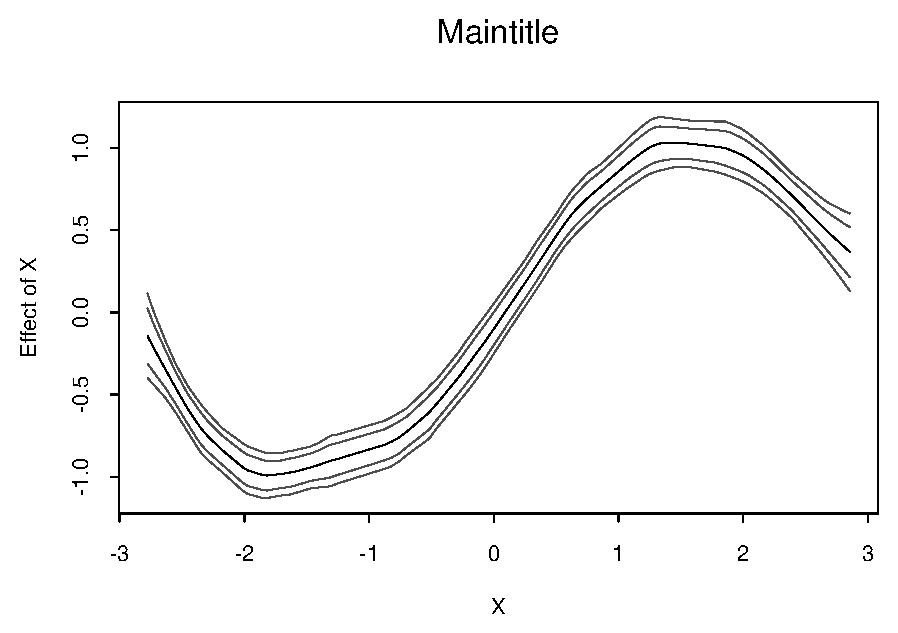
\includegraphics[scale=0.8]{grafiken/remlregplotnonp.eps}
{\em \caption{ \label{remlregillgraph} Illustration for the usage
of \em\texttt{plotnonp}}}
\end{center}
\end{figure}

In some situations the effect of a covariate representing dates
must be plotted. Suppose for example that a covariate has values
ranging from 1 to 19 representing the time period from January
1983 to July 1984. In this case, we naturally prefer that the
x-axis is labelled in terms of dates rather than in the original
coding (from 1 to 19). To achieve this, function #plotnonp#
provides the three additional options #year#, #month# and #step#.
Options #year# and #month# are  used to specify the year and the
month (1 for January, 2 for February, \dots) corresponding to the
minimum covariate value. In the example mentioned above
#year=1983# and #month=1# will produce the correct result. In
addition, option #step# may be specified to define the periodicity
in which your data are collected. For example #step=12# (the
default) corresponds to monthly data, while #step=4#, #step=2# and
#step=1# correspond to quarterly, half yearly and yearly data. We
illustrate the usage of #year#, #month# and #step# with our
example. Suppose we estimated the effect of calendar time #D#,
say, on a certain dependent variable, where the range of the data
is as described above. Then the following S-plus function call
will produce the postscript file shown in
\autoref{remlregillgraph2}:

#> plotnonp("c:\\bayes\\r_f_D_pspline.res", psname="c:\\bayes\\r_f_D_pspline.ps",#\\
#  year=1983,month=1,step=12,xlab="date", ylab=" ")#

\begin{figure}[ht]
\begin{center}
%\includegraphics[scale=0.8]{fvdate.eps}
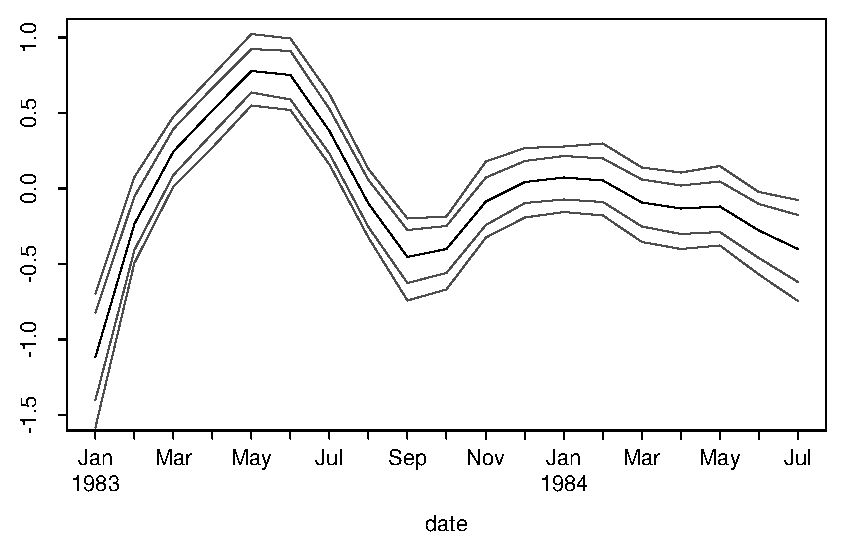
\includegraphics[scale=0.8]{grafiken/plotnonpdate.eps}
{\em \caption{ \label{remlregillgraph2} Illustration for the usage
of \em\texttt{plotnonp}}}
\end{center}
\end{figure}

Note, that \texttt{ylab=" "} forces S-plus to omit the y axis
label. If ylab (as well as xlab) is omitted, default labels will
be given to the two axis.

Finally, we note that all options that can be passed to the #plot#
function of S-plus may also be passed to function #plotnonp#.
Thus, function #plotnonp# is more or less a specialized version of
the S-plus #plot# function.

\subsubsection{Drawing geographical maps}
\index{S-plus!drawing geographical maps} \index{drawing
geographical maps}

This subsection describes how to visualize estimation results of
spatial covariates, where the observations represent the location
or site in connected geographical regions. A typical example for a
spatial covariate is given in the 'rents for flats' example, see
\autoref{rentdata},  where the covariate #L# indicates the
location (in subquarters) of the flat in Munich.
\autoref{remlregmunich} shows a map of Munich separated into
subquarters.

\begin{figure}
\centering
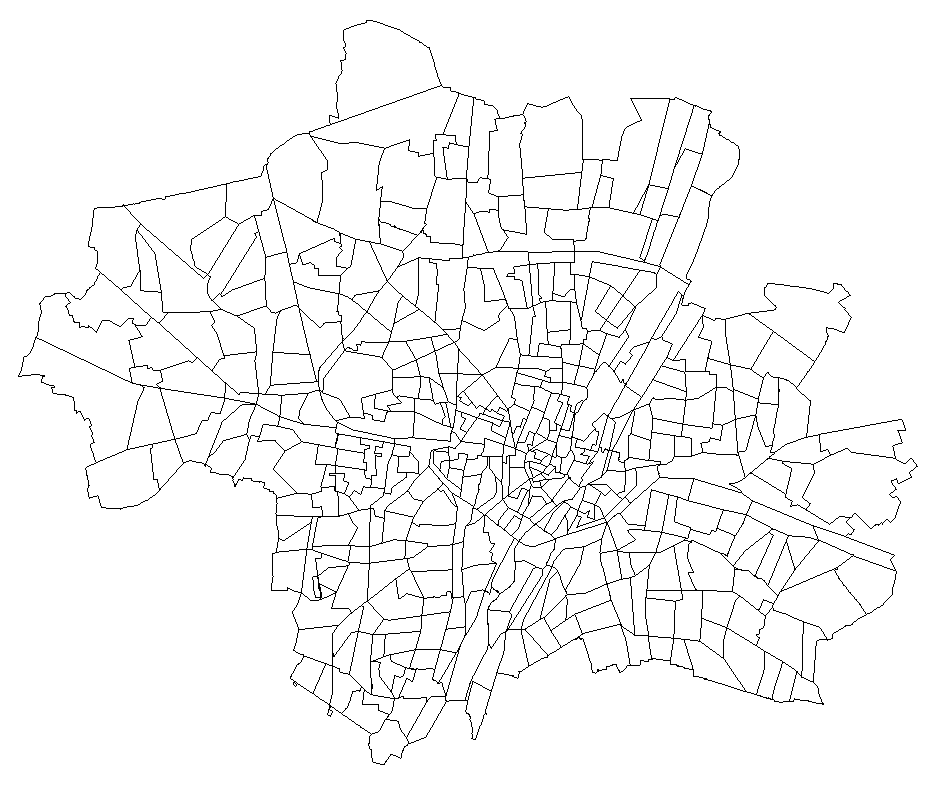
\includegraphics [scale=0.5]{grafiken/munich.eps}
{\em \caption{\label{remlregmunich} Map of Munich}}
\end{figure}

Typically, the effect of such a spatial covariate is incorporated
into a regression model via an unstructured or structured random
effect. In the latter case a spatial smoothness prior for the
spatial covariate is specified that penalizes too abrupt changes
of the estimated effect in neighboring sites. In some situations
the incorporation of both, an unstructured and a structured
effect, may also be appropriate. Details on how to incorporate
spatial covariates into a semiparametric regression  model are
given in \autoref{remlregregress}. For the rest of this section we
assume that an effect of a spatial covariate has already been
estimated and that we want to visualize the estimation results.
This can easily be done with the two S-plus functions
#readbndfile# and #drawmap#. Function #readbndfile# is used to
read the boundary information of a map that is stored in a
boundary-file and to store this information as a permanent S-plus
{\em map object}. The boundary file contains mainly the polygons which
form the different geographical regions of the map. The required
structure of such a file is described in \autoref{map}. After the
successful reading of the boundary information of a map, the
second function #drawmap# may be used to draw and print the map
either on the screen or into a postscript file. There are several
possible ways to draw the map. In the simplest case the map can be
drawn without any estimation effects, i.e. only the boundaries of
the different regions or sites are drawn, see
\autoref{remlregmunich} for an example. In practice, however, one
usually wants to color the regions of the map according to some
numerical characteristics. As an example compare
\autoref{remlregmunichrelfreq} in which the subquarters of Munich
are colored according to the frequency of flats in the rent data
set located in the respective subquarter. Subquarters colored in
red contain less flats compared to subquarters colored in green.
In striped areas no observations are available.

\begin{figure}[ht]
\begin{center}
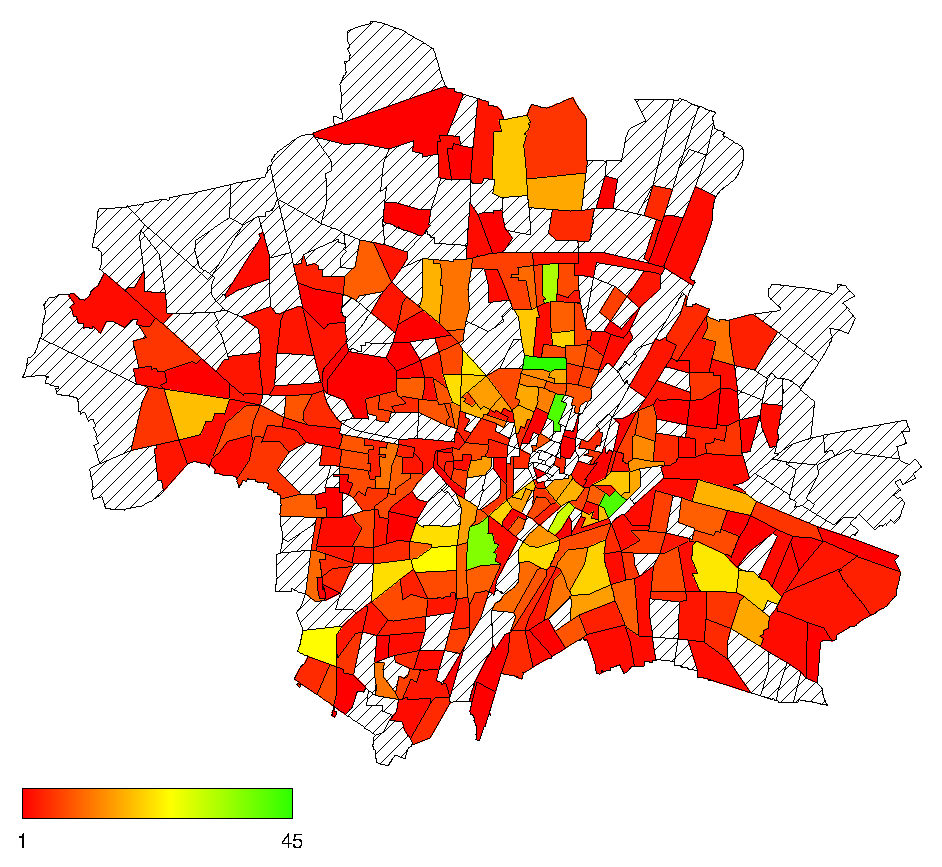
\includegraphics[scale=0.5]{grafiken/munichfr.eps}
{\em \caption{ \label{remlregmunichrelfreq} relative frequencies
of observed flats in the 'rents for flats' data set}}
\end{center}
\end{figure}


In the following we give a detailed description of the usage of
the functions #readbndfile# and #drawmap#.

{\bf Function readbndfile}
\medskip
\index{S-plus!reading boundary files} \index{reading boundary
files}

Function #readbndfile# is used to read in boundary information
stored in a boundary file into S-plus. The function has two
required arguments. The first argument is the file name of the
boundary file to read in. The second argument specifies the name
of the {\em map object} in S-plus (recall that the map information
is stored as a permanent S-plus object). To give an example,
suppose that {\em BayesX} is installed in the directory
\texttt{c:$\backslash$bayes} and that we want to read in the map
of Munich. In this case the boundary file of the map is stored in
the subdirectory #examples# of the installation directory, that is
in \texttt{c:$\backslash$bayes$\backslash$examples}. The name of
the boundary file is #munich.bnd#. The following function call
reads in the boundary information of Munich and stores the map
permanently in S-plus:

#> readbndfile("c:\\bayes\\examples\\munich.bnd","munich")#

Once again, note that double backslashes are required in S-plus to
specify a directory. The second argument in the statement above is
#"munich"#, i.e. the name of the {\em map object} is simply
#munich#. To refer to the map of Munich in subsequent statements
and function calls, the quotation marks must be omitted.

{\bf Function drawmap}
\medskip
\index{S-plus!drawmap}

Function #drawmap# is used to draw geographical maps and color the
regions according to some numerical characteristics. The only
required argument that must be passed to #drawmap# is the name of
the map to be drawn. Provided that the map has already been read
into S-plus (via function #readbndfile#), the following statement
draws the map of Munich in a S-plus graphic-window on the screen:

#> drawmap(map=munich)#

Storing the map in a postscript file rather than drawing it on the
screen can be achieved by specifying the name of the postscript
file using the #outfile# option. For example the command

#> drawmap(map=munich,outfile="c:\\bayes\\munich.ps")#

produces a postscript file named #munich.ps# with the map of
Munich.

However, in most cases one does not only want to draw the
boundaries of a geographical map, but also to color the regions
according to some numerical characteristics. Suppose for example
that we have already estimated a location specific effect on the
monthly rents in the 'rents for flats' data set. Suppose further
that the estimated effects are stored in
\texttt{c:$\backslash$bayes$\backslash$output$\backslash$r\_f\_L\_spatial.res}.
The structure of the file is described in detail in
\autoref{remlregregress}.

Suppose now that we want to visualize estimation results for the
spatial covariate location by coloring the subquarters of Munich
according to the estimated posterior mode. Compared to the S-plus
statement above, (at least) three more arguments must be passed to
function  #drawmap#; the argument #dfile# that specifies the file
name of estimated results, the argument #plotvar# that specifies
the variable to be plotted and the argument #regionvar# that
specifies which column of the file stores the region names. The
following statement produces the desired result:

#> drawmap(map=munich,outfile="c:\\bayes\\munich.ps", plotvar="pmode",regionvar="L", #\\
#  dfile="c:\\bayes\\output\\b_f_L_spatial.res")#

Note that the right hand side of options #plotvar# and #regionvar#
must be enclosed by quotation marks.

{\bf Optional arguments of function drawmap}

Besides the arguments discussed so far there are some more
optional arguments that can be passed to #drawmap#. They are
listed and described below together with a summary of the
arguments that have already been mentioned:


\begin{itemize}
\item {\bf map = mapname}

Name of the S-plus {\em map object}. Use function #readbndfile# to read
in geographical maps into S-plus. \item {\bf dfile = "filename
(including path)"}

Name (including path) of the file containing numerical
characteristics of the regions of the map. The file must contain
at least two columns, one column that lists the names of the
regions and one column containing the numerical characteristics of
the respective regions. It is important that the names of the
regions match with the region names stored in the S-plus {\em map
object}. The first row of the file must contain the names of the
columns.
\item {\bf outfile = "filename (including path)"}

Name (including path) of the postscript file where the map should
be stored.
\item {\bf regionvar = "characterstring"}

Name of the column in the data file containing the region names
(see also argument #dfile#). Note that the right hand side must be
enclosed by quotation marks. \item {\bf plotvar = "characterstring"}

Name of the column in the data file containing the numerical
characteristics of the regions (see also argument #dfile#). Note
that the right hand side must be enclosed by quotation marks.
\item {\bf lowerlimit = realvalue}

Lower limit of the range to be drawn. If #lowerlimit# is omitted,
the minimum numerical value in the #plotvar# column will be
used as the lower limit. \item {\bf upperlimit = realvalue}

Upper limit of the range to be drawn. If #upperlimit# is omitted,
the maximum numerical value in the #plotvar# column will be
used as the upper limit. \item {\bf nrcolors = integer}

To color the regions according to their numerical characteristics,
the data are divided into a (typically large) number of ordered
categories. Afterwards a color is associated with each category.
The #nrcolors# option can be used to specify the number of
categories (and with it the number of different colors). The
default value is #nrcolors=100#. \item {\bf pstitle = "characterstring"}

Adds a title to the graph. Note that the right hand side must be
enclosed by quotation marks.
\item {\bf color = T/F}

The #color# option allows to choose between a grey scale for the
colors and a colored scale. The default is #color=F#, which means
a grey scale. \item {\bf legend = T/F}

By default a legend is drawn into the graph. To omit the legend in
the graph, #legend=F# must be passed as an additional argument.
\item {\bf drawnames = T/F}

In some situations it may be favorable to print the names of the
regions into the graph (although the result may be confusing in
most cases). This can be done by specifying the additional option
#drawnames=T#. By default the names of the regions are omitted in
the graph. \item {\bf swapcolors = T/F}

In some situations it may be favorable to swap the order of the
colors, i.e. red shades corresponding to large values and green
shades corresponding to small values. This is achieved by
specifying #swapcolors=T#. By default small values are colored in
red shades and large values in green shades. \item {\bf pcat =
T/F}

If you want to visualize the values of the columns #pcat80# or
#pcat95# it is convenient to specify #pcat=T#. This forces
#drawmap# to expect a column that consists only of the values -1,
0 and 1. Of course you can achieve the same result by setting
#nrcolors=3#, #lowerlimit=-1# and #upperlimit=1#. The default is
#pcat=F#.
\end{itemize}

\subsubsection{Plotting 2 dimensional surfaces}

This subsection describes the usage of the function #plotsurf# for
visualizing 2 dimensional surfaces. The function #plotsurf# merely
invokes different S-plus functions for visualizing 2 dimensional
data. Thus, users familiar with S-plus may prefer to use this
functions directly to gain more flexibility. Note that this function
is only available for S-plus.

Suppose that a Bayesian regression model has already been
estimated with predictor

$$
\eta = \dots + f(X1,X2) + \dots,
$$

where the interaction effect of #X1# and #X2# is modelled
nonparametrically using 2 dimensional P-splines and that the
estimation results are stored in file:

#c:\bayes\output\r_f_X1_X2_pspline.res#

The S-plus function #plotsurf# requires at least one argument,
which is the name (including path) of the file containing the
estimation results. For example the command

#plotsurf("c:\\bayes\\output\\b_f_X1_X2_pspline.res")#

prints the posterior mode against X1 and X2 on the screen. There
are several additional options that can be passed, for example for
changing the plot type or storing the graph as a postscript file
rather than displaying it on the screen. The following list
describes all possible arguments that may be passed to the
function #plotsurf#:

\begin{itemize}
\item {\bf data = "filename (including path)"}

Name (including path) of the file containing the estimation
results. The file must contain at least 3 columns, one for the
x-axis, one for the y-axis and one for the z-axis. The file must
contain a header.
\item {\bf outfile = "filename (including path)"}

Name (including path) of the postscript file where the graph
should be stored. This option is only meaningful for #mode=2# and
#mode=3#. \item {\bf cols = 3 column vector}

This option is only meaningful, if the argument #data# is
specified. In this case #cols# gives the columns of the object or
data file passed to the argument #data# that should be used as
values for the x, y and z axis. The default is #cols=c(2,3,4)#
which corresponds to plotting the posterior mode against #X1# and
#X2#.
%\item {\bf zlim = 2 column vector}

%2 column vector giving the minimum and maximum value to be put on
%the z-axis.
\item {\bf mode = 1/2/3/4/5}

This option specifies the plot type. Currently 5 different types
are available. The default is #mode=1#, which corresponds to what
is called a 'Surface Plot' in S-plus.
\end{itemize}


\section{Global options}
\label{remlregglobopt} \index{remlreg object!global options}

The purpose of global options is to affect the global behavior of
a {\em remlreg object}. The main characteristic of global options
is, that they are not associated with a certain method.

The syntax for specifying global options is

{\em objectname}.{\em optionname} = {\em newvalue}

where {\em newvalue} is the new value of the option. The type of
the value depends on the respective option.

Currently only one global option is available for {\em remlreg
objects}:

\begin{itemize}
\item {\bf outfile = filename} \\
By default, the estimation output produced by the #regress#
procedure will be written to the default output directory, which
is

#<#INSTALLDIRECTORY#>\output#.

The default file name is composed of the name of the {\em remlreg
object} and the type of the file. For example, if you estimated a
nonparametric effect for a covariate #X#, say, using P-spline then
the estimation output will be written to

#<#INSTALLDIRECTORY#>\output\r_f_X_pspline.res#

where #r# is the name of the {\em remlreg object}. In most cases,
however, it may be necessary to save estimation results into a
different directory and/or under a different file name than the
default. This can be done using the #outfile# option. With the
outfile option you have to specify the directory where the output
should be stored to and in addition a base file name. The base
file name should not be a complete file name. For example specifying

#outfile = c:\data\res1#

would force {\em BayesX} to store the estimation result for the
nonparametric effect of #X# in file

#c:\data\res1_f_X_pspline.res#
\end{itemize}

\section{Examples}
\label{remlregexamples}

\subsection{Determinants of childhood undernutrition in Zambia}
\label{remlregzambianalysis}

To make the user familiar with the usage of {\em remlreg objects}
we present a tutorial like example in this subsection. We use data
on undernutrition of children in Zambia, compare \autoref{zambia}
for a description of the data set. The files containing the data
and the map can be found in the subdirectory #examples# of the
installation directory together with the batch file
#remltutorial.prg# containing all commands used in the following
subsections.

The rest of the example is organized as follows: In
\autoref{zambia_reml_datasets} we create a {\em dataset object} to
incorporate, handle and manipulate the data. We will also give a
brief description of some methods that may be applied to {\em
dataset objects}. Since we want to estimate a spatial effect of
the district in which a child lives, we need the boundaries of the
districts to compute the neighborhood information of the map of
Zambia. This information will be stored in a {\em map object}.
\autoref{zambia_reml_maps} describes how to create
and handle these objects. Estimation of the regression model is
carried out in \autoref{zambia_reml_regression} using a {\em
remlreg object}. The last two subsubsections describe how to
visualize the estimation results and how to customize the obtained
graphics.

Please note, that all paths within the following subsections must
be changed according to the storage location of the corresponding
files on your hard disk.

\subsubsection{Reading data set information}\label{zambia_reml_datasets}

In a first step we read the available data set information into
{\it BayesX}. Therefore we create a {\it dataset object} named
#d#:

#> dataset d#

We store the data in #d# using the method #infile#:

#> d.infile, maxobs=5000 using c:\data\zambia.raw#

Note, that we assume the data to be provided in the external file
#c:\data\zambia.raw#. The first few lines of this file look like
this:

{\footnotesize
 hazstd bmi agc district rcw edu1 edu2 tpr sex\\
 0.0791769 \,\, 21.83 \,\, 4 \,\, 81 \,\, -1 \,\, 1 \,\, 0 \,\, 1 \,\, -1\\
 -0.2541965 \,\, 21.83 \,\, 26 \,\, 81 \,\, -1 \,\, 1 \,\, 0 \,\, 1 \,\, -1\\
 -0.1599823 \,\, 20.43 \,\, 56 \,\, 81 \,\, 1 \,\, -1 \,\, -1 \,\, 1 \,\, 1\\
 0.1733911 \,\, 22.27 \,\, 6 \,\, 81 \,\, -1 \,\, 0 \,\, 1 \,\, 1 \,\, 1}

In our example the file contains the variable names in the first
line. Therefore  it is not necessary to specify them in the
#infile# command. If the file contained only the data without
variable names, we would have to supply them after the keyword
#infile#:

 #> d.infile hazstd bmi agc district rcw edu1 edu2 tpr sex, maxobs=5000#\\
 #  using c:\data\zambia.raw#


Option #maxobs# can be used to speed up the execution time of the
#infile# command. If #maxobs# is specified, {\it BayesX} allocates
enough memory to store all the data while the total amount of
required memory is unknown in advance if #maxobs# remains
unspecified. For larger data sets this may cause {\it BayesX} to
start reading the data set information several times because the
currently allocated memory is exceeded. However, this is only
meaningful for larger data sets with more than 10,000 observations
and could therefore be omitted in our example.

A second option that may added to the {\tt infile} command is the
{\tt missing} option to indicate missing values. Specifying for
example {\tt missing = M} defines the letter 'M' as an
indicator for a missing value. The default for missing values are
a period '.' and 'NA' (which remain valid indicators for
missing values even if an additional indicator is defined by the
{\tt missing} option).

After having read in the data set information we can inspect the
data visually. Executing the command

#> d.describe#

opens an {\it Object-Viewer} window containing the data in form of
a spreadsheet. This can also be achieved by double-clicking on the
{\it dataset object} in the {\it object browser}.

Further methods allow to examine the variables in the {\it dataset
object}. For a categorial variable, e.g.~#sex#, the #tabulate#
command may be used to produce a frequency table:

#> d.tabulate sex#

resulting in

\begin{verbatim}
Variable: sex

          Value       Obs           Freq            Cum
             -1      2451         0.5057         0.5057
              1      2396         0.4943              1
\end{verbatim}

being printed in the {\it output window}. For continuous variables
the #descriptive# command prints several characteristics of the
variable in the {\em output window}. E.g., executing

#> d.descriptive bmi#

leads to

\begin{verbatim}
   Variable    Obs        Mean      Median         Std         Min         Max
        bmi   4847   21.944349        21.4   3.2879659        12.8       39.29
\end{verbatim}

\subsubsection{Map objects}\label{zambia_reml_maps}

In the following we want to estimate a spatially correlated effect
of the district in which a child lives. Therefore we need the
boundaries of the districts in Zambia to compute the neighborhood
information of the map of Zambia. We therefore create a {\it map
object}

#> map m#

and read in the boundaries using the #infile# command of {\it map
objects}:

#> m.infile using c:\data\zambia.bnd#

Having read in the boundary information, {\it BayesX}
automatically computes the neighborhood matrix of the map.

The file following the keyword #using# is assumed to contain the
boundaries in form of closed polygons. Compare \autoref{map} for a
description of the expected file format.

{\it Map objects} may be visualized using method #describe#:

#> m.describe#

resulting in the graph shown in \autoref{zambia_reml_zambiamap}.
Additionally, #describe# prints further information about the {\it
map object} in the {\it output window} including the name of the
object, the number of regions, the minimum and maximum number of
neighbors and the bandwidth of the corresponding adjacency or
neighborhood matrix:

\begin{verbatim}
  MAP m
  Number of regions: 54
  Minimum number of neighbors: 1
  Maximum number of neighbors: 9
  Bandsize of corresponding adjacency matrix: 24
\end{verbatim}

\begin{figure}[ht]
\begin{center}
\epsfig{file=grafiken/zambia.ps,scale=0.35} {\it\caption{The districts
within Zambia.\label{zambia_reml_zambiamap}}}
\end{center}
\end{figure}

Reading the boundary information from an external file and
computing the neighborhood matrix may be a computationally
intensive task if the map contains a huge number of regions or if
the polygons are given in great detail. To avoid doing these
computations every time {\em BayesX} is restarted, we may store
the computed neighborhood information in a so-called {\it graph
file} to make it directly available (compare \autoref{map} for the
structure of a graph file). To do this, we use the method
#outfile# together with the #graph# option as in the following
example:

#> m.outfile, replace graph using c:\data\zambia.gra#

Note, that specifying the option #replace# allows {\it BayesX} to
overwrite an existing file with the same name. Without this option
an error message would be raised if the given file is already
existing. Leaving out the keyword #graph# in the above command
leads to storage of the map in boundary format.

To see how storing maps in {\it graph files} affects the
computation time of the #infile# command, we create a second {\it
map object} and read in the information from the graph file.
Again, we have to specify the keyword #graph#:

\begin{verbatim}
> map m1
> m1.infile, graph using c:\data\zambia.gra
\end{verbatim}

As you should have noticed, reading geographical information from
a {\it graph file} is usually much faster than reading from a {\it
boundary file}. However, using {\it graph files} also has a
drawback. Since they do no longer contain the full information on
the polygons forming the map, we can not visualize a {\it map
object} created from a {\it graph file}. Trying to do so

#> m1.describe#

raises an error message. This implies, that visualizing estimation
results of spatial effects can only be based on {\it map objects}
created from {\it boundary files}, although estimation can be
carried out using {\it graph files}. Since we will work with the
{\it map object} #m# in the following, we delete #m1#:

#> drop m1#

\subsubsection{Bayesian semiparametric
regression}\label{zambia_reml_regression}

To estimate a regression model based on mixed model techniques, we
first create a {\it remlreg object}:

#> remlreg r#

By default estimation results are written to the subdirectory
#output# of the installation directory. In this case the default
filenames are composed of the name of the {\it remlreg object} and
the type of the specific file. Usually it is more convenient to
store the results in a user-specified directory. To define this
directory we use the #outfile# command of {\it remlreg objects}:

#> r.outfile = c:\data\r#

Note, that #outfile# does not only specify a directory but also a
base file name (the character 'r' in our example). Therefore
executing the command above leads to storage of the results in the
directory #c:\data# and all filenames start with the character
'r'. Of course the base file name may be different from the name of
the {\it remlreg object}.

In addition to parameter estimates {\it BayesX} also produces some
further information on the estimation process. In contrast to
parameter estimates this information is not stored automatically
but is printed in the {\it output window}. Therefore it is useful
to store the contents of the {\it output window}. This can be
achieved automatically by opening a {\it log file} using the
#logopen# command

#> logopen, replace using c:\data\logreml.txt#

After opening a {\it log file}, every information written to the
{\em output window} is also stored in the log file. Option
#replace# allows {\it BayesX} to overwrite an existing file with
the same name as the specified {\it log file}. Without #replace#
results are appended to an existing file.

The model presented in Kandala et al. (2001) is given by the
following semiparametric predictor:
\[\eta=\gamma_0+\gamma_1rcw+\gamma_2edu1+\gamma_3edu2+\gamma_4tpr+\gamma_5sex+f_1(bmi)+f_2(agc)+f^{str}(district)+f^{unstr}(district)\]
The two continuous covariates #bmi# and #agc# are assumed
to have a possibly nonlinear effect on the Z-score and are
therefore modelled nonparametrically (as P-splines with second
order random walk prior in our example). The spatial effect of the
district is split up into a spatially correlated part $
f^{str}(district)$ and an uncorrelated part $f^{unstr}(district)$,
see Fahrmeir and Lang (2001b) for a motivation. The correlated
part is modelled by a Markov random field prior, where the
neighborhood matrix and possible weights associated with the
neighbors are obtained from the {\it map object} #m#. The
uncorrelated part is modelled by an  i.i.d.~Gaussian effect.

To estimate the model we use method #regress# of {\em remlreg
objects}:
\begin{verbatim}
> r.regress hazstd = rcw + edu1 + edu2 + tpr + sex + bmi(psplinerw2)
  + agc(psplinerw2) + district(spatial,map=m) + district(random),
  family=gaussian lowerlim=0.01 eps=0.0005 using d
\end{verbatim}

Options #lowerlim# and #eps# control the estimation process. Since
small variances are near to the boundary of their parameter space,
the usual Fisher-scoring algorithm for their determination has to
be modified. If the fraction of the penalized part of an effect
relative to the total effect is less than #lowerlim#, the
estimation of the corresponding variance is stopped and the
estimator is defined to be the current value of the variance (see
chapter 7 in the manual for details). The option #eps# defines the
termination criterion for the estimation process. The default
values are #lowerlim=0.001# and #eps=0.00001#. However, since our
analysis is only for explanatory purpose we chose somewhat weaker
conditions resulting in a faster 'convergence' of the algorithm.
On a 2.4 GHz PC estimation of our model took about 2 minutes and
30 seconds with the above specifications of #lowerlim# and #eps#.

A further option of method #regress# is #maxit#, defining the
maximum number of iterations that should be performed in the
estimation. Note, that {\it BayesX} produces results based on the
current values of all parameters even if no convergence could be
achieved within #maxit# iterations. In this case however a warning
message will be printed in the {\it output window}.

In the following we reproduce the content of the {\em output
window} to make the user familiar with the estimation results
produced by {\em BayesX}:

\footnotesize
\begin{verbatim}
ESTIMATION RESULTS:

  Estimated scale parameter: 0.802145

  Scale parameter is also stored in file
  c:\data\r_scale.res


  f_bmi_pspline

  Estimated variance:  1.14816e-05
  Inverse variance:    87095.9
  Smoothing parameter: 69863.5
  (Smoothing parameter = scale / variance)
  NOTE: Estimation of the variance was stopped after iteration 6
        because the corresponding penalized part was small relative to the linear predictor.

  Variance and smoothing parameter are stored in file
  c:\data\r_f_bmi_pspline_var.res

  Results are stored in file
  c:\data\r_f_bmi_pspline.res

  Postscript file is stored in file
  c:\data\r_f_bmi_pspline.ps

  Results may be visualized using method 'plotnonp'
  Type for example: objectname.plotnonp 1


  f_agc_pspline

  Estimated variance:  0.00322146
  Inverse variance:    310.418
  Smoothing parameter: 249
  (Smoothing parameter = scale / variance)

  Variance and smoothing parameter are stored in file
  c:\data\r_f_agc_pspline_var.res

  Results are stored in file
  c:\data\r_f_agc_pspline.res

  Postscript file is stored in file
  c:\data\r_f_agc_pspline.ps

  Results may be visualized using method 'plotnonp'
  Type for example: objectname.plotnonp 2


  f_district_spatial

  Estimated variance:  0.0294012
  Inverse variance:    34.0123
  Smoothing parameter: 27.2828
  (Smoothing parameter = scale / variance)

  Variance and smoothing parameter are stored in file
  c:\data\r_f_district_spatial_var.res

  Results are stored in file
  c:\data\r_f_district_spatial.res

  Postscript file is stored in file
  c:\data\r_f_district_spatial.ps

  Results may be visualized in BayesX using method 'drawmap'
  Type for example: objectname.drawmap 3



  f_district_random

  Estimated variance:  0.00806668
  Inverse variance:    123.967
  Smoothing parameter: 99.4393
  (Smoothing parameter = scale / variance)

  Variance and smoothing parameter are stored in file
  c:\data\r_f_district_random_var.res

  Results for random effects are stored in file
  c:\data\r_f_district_random.res


  FixedEffects

  Variable  Post. Mode     Std. Dev.      p-value        95% Confidence Interval
  const     0.0610357      0.0341574      0.0367456      -0.00592622    0.127998
  rcw       0.00767158     0.0136564      0.286931       -0.0191003     0.0344434
  edu1      -0.0605105     0.0261369      0.0103181      -0.111749      -0.00927192
  edu2      0.234917       0.0459925      4.41249e-06    0.144754       0.325081
  tpr       0.0904093      0.0218891      6.17648e-05    0.047498       0.133321
  sex       -0.0585716     0.0129304      2.04243e-05    -0.0839203     -0.0332229

  Results for fixed effects are also stored in file
  c:\data\r_FixedEffects.res


  Additive predictor and expectations

  Additive predictor and expectation for each observation are stored in file
  c:\data\r_predict.raw

  Files of model summary:

  ---------------------------------------------------------------------------

  Batch file for visualizing effects of nonlinear functions is stored in file
  c:\data\r_graphics.prg

  NOTE: 'input filename' must be substituted by the filename of the boundary-file

  ---------------------------------------------------------------------------

  Batch file for visualizing effects of nonlinear functions
  in S-Plus is stored in file
  c:\data\r_splus.txt

  NOTE: 'input filename' must be substituted by the filename of the boundary-file

  ---------------------------------------------------------------------------

  Latex file of model summaries is stored in file
  c:\data\r_model_summary.tex

  ---------------------------------------------------------------------------
\end{verbatim}
\normalsize

In addition to the information being printed to the {\em output
window} results for each effect are written to external ASCII
files. The names of these files are given in the {\em output
window}, compare the previous pages. For the variance parameters
the files contain the variance as well as the corresponding
smoothing parameter. For the different terms of the model the
files contain the posterior mode, the 80\% and 95\% credible
interval, the standard deviations and the corresponding 95\% and
80\% posterior probabilities of the estimated effects. Note, that
credible intervals and posterior probabilities are based on a
normal approximation of the posterior. For example, the beginning
of the file #c:\data\r_f_bmi_pspline.res# for the effect of #bmi#
looks like this:

{\footnotesize
 intnr \,\, bmi \,\, pmode \,\, ci95lower \,\, ci80lower \,\, std \,\, ci80upper \,\, ci95upper \,\, pcat95 \,\, pcat80\\
 1 \,\, 12.8 \,\, -0.22305 \,\, -0.304661 \,\, -0.276409 \,\, 0.0416301 \,\, -0.169692 \,\, -0.141439 \,\, -1 \,\, -1\\
 2 \,\, 13.15 \,\, -0.215246 \,\, -0.292828 \,\, -0.26597 \,\, 0.0395749 \,\, -0.164522 \,\, -0.137663 \,\, -1 \,\, -1\\
 3 \,\, 14.01 \,\, -0.19607 \,\, -0.264173 \,\, -0.240597 \,\, 0.0347394 \,\, -0.151544 \,\, -0.127968 \,\, -1 \,\, -1}

The credible intervals and posterior probabilities that are
computed for every effect may be changed by the user using the
options #level1# and #level2#. For example specifying #level1=99#
and #level2=70# in the option list of the #regress# command leads
to the computation of 70\% and 99\% credible intervals and
posterior probabilities. The defaults are #level1=95# and
#level2=80#.

Some nonparametric effects are visualized by {\em BayesX}
automatically and the resulting graphs are stored in postscript format.
E.g.~the effect of #bmi# is visualized in the file
#c:\data\b_f_bmi_pspline.ps# (compare the results on the previous
pages for the other filenames). A batch file to reproduce the
plots is stored in the output directory. In our example the name
of the file is #c:\data\r_graphics.prg#. The advantage is that
additional options may be added by the user to customize the
graphs (compare the following two subsubsections).

Moreover a file with ending #.tex# is created in the outfile
directory. This file contains a summary of the estimation results
and may be compiled using \LaTeX.

Having finished the estimation we may close the {\it log file} by
typing

#> logclose#

Note, that the {\it log file} is closed automatically when you
exit {\em BayesX}.

\subsubsection{Visualizing estimation results}\label{zambia_reml_visual}

{\em BayesX} provides three possibilities to visualize estimation
results:
\begin{itemize}
\item As mentioned in the previous subsubsection, certain results are
automatically visualized by {\em BayesX} and stored in postscript
files.
\item Post estimation commands of {\em bayesreg objects} allow to
visualize results after having executed a #regress# command.
\item {\em Graph objects} may be used to produce graphics using the ASCII files containing the estimation results.
In principle {\em graph objects} allow the visualization of any
content of a {\em dataset object}. {\em Graph files} are also used
in the batch file containing the commands to reproduce the
automatically generated graphics.
\end{itemize}

In this subsubsection we describe the general usage of the post
estimation commands as well as the commands for the usage with
{\em graph objects} to enable the user to reproduce the
automatically generated plots directly in {\em BayesX}.
\autoref{zambia_reml_custom} describes how to customize plots.

\paragraph{Post estimation commands}

After having estimated a regression model plots for nonparametric
effects of metrical covariates can be produced using the post
estimation command #plotnonp#:

#> r.plotnonp 1#

and

#> r.plotnonp 2#

produce the graphs shown in \autoref{zambia_reml_bmi1} in an {\it
object-viewer window}. The numbers following the #plotnonp#
command depend on the order in which the model terms have been
specified. The numbers are supplied in the {\em output window}
after estimation, compare the results in the previous
subsubsection.

By default the plots contain the posterior mode and pointwise
credible intervals according to the levels specified in the
#regress# command. So by default the plots include pointwise 80\%
and 95\% credible intervals.

\begin{figure}[ht]
\begin{center}
\epsfig{file=grafiken/zambia_reml_f_bmi1.ps,scale=0.5}
\epsfig{file=grafiken/zambia_reml_f_age1.ps,scale=0.5} {\it\caption{Effect
of the body mass index of the child`s mother and of the age of the
child together with pointwise 80\% and 95\% credible intervals.
\label{zambia_reml_bmi1}}}
\end{center}
\end{figure}

A plot may be stored in postscript format using the #outfile# option.
Executing

#> r.plotnonp 1, replace outfile = c:\data\f_bmi.ps#

stores the plot for the estimated effect of #bmi# in the file
#c:\data\f_bmi.ps#. Again, specifying #replace# allows {\it
BayesX} to overwrite an existing file. Note, that {\it BayesX}
does not display the graph on the screen if the option #outfile#
is specified.

Estimation results for spatial effects are best visualized by
drawing the respective map and coloring the regions of the map
according to some characteristic of the posterior, e.g. the
posterior mode. For the structured spatial effect this can be
achieved using the post estimation command #drawmap#

#> r.drawmap 3#

which results in the graph shown in \autoref{zambia_reml_spat1}.

\begin{figure}[ht]
\begin{center}
\epsfig{file=grafiken/zambia_reml_f_spat1.ps,scale=0.35}
{\it\caption{Posterior mode of the structured spatial
effect.\label{zambia_reml_spat1}}}
\end{center}
\end{figure}


\paragraph{Graph Objects}

The commands presented in the previous paragraph work only after
having estimated a regression model in the current {\em BayesX} session
but it may also be useful to visualize results of former analyzes.
This can be achieved using {\em graph objects}. Note again, that
{\em graph files} are also used in the batch file containing the
commands to reproduce the automatically generated graphics.
Therefore the purpose of this paragraph is also to enable the user
to understand the content of this batch file.

First we read the estimation results into a {\it dataset object}.
For example the estimation results for the effect of #bmi# can be
read into {\it BayesX} by executing the commands

\begin{verbatim}
> dataset res
> res.infile using c:\data\r_f_bmi_pspline.res
\end{verbatim}

Now the estimation results (or any content of a {\it dataset
object}) may be visualized using a {\it graph object} which we
create by typing

#> graph g#

The results stored in the {\em dataset object} #res# are now
visualized using the #plot# command of {\it graph objects}.
Executing

 #> g.plot bmi pmode ci95lower ci80lower ci80upper ci95upper using res#

reproduces the graph in \autoref{zambia_reml_bmi1}.

Similar as for #plotnonp#, the direct usage of the #drawmap#
command is only possible after executing a #regress# command.
However, using {\it graph objects} again allows us to visualize
results that have been stored in a file.

First we read the information contained in this file into a {\it
dataset object}. For example the following command

#> res.infile using c:\data\r_f_district_spatial.res#

stores the estimation results for the structured spatial effect in
the {\em dataset object} #res#. Now we can visualize the posterior
mode using method #drawmap# of {\it graph objects} leading again
to the graph shown in \autoref{zambia_reml_spat1}:

#> g.drawmap pmode district, map=m using res#

Since -- in contrast to a {\it remlreg object} -- no {\it map
object} is associated with a {\it graph object}, we explicitly
have to specify the map that we want to use in the option list.

Using {\it graph objects} also allows us to plot other
characteristics of the posterior than the posterior mode. For
instance the posterior 95\% probabilities may be visualized by

#> g.drawmap pcat95 district, map=m using res#

The result is shown in \autoref{zambia_reml_spat2}.

\begin{figure}[ht]
\begin{center}
\epsfig{file=grafiken/zambia_reml_f_spat2.ps,scale=0.35}
{\it\caption{Posterior 95\% probability of the structured spatial
effect.\label{zambia_reml_spat2}}}
\end{center}
\end{figure}

A further advantage of {\it graph objects} is, that they allow to
visualize the estimation results for the uncorrelated spatial
effects. Since these are modelled as unstructured random effects,
{\it BayesX} is unable to recognize them as spatial effects.
However, proceeding as follows gives us the possibility to plot
the unstructured spatial effect shown in
\autoref{zambia_reml_random1}:

\begin{verbatim}
> res.infile using c:\data\r_f_district_random.res
> g.drawmap pmode district, map=m color swapcolors using res
\end{verbatim}

\begin{figure}[ht]
\begin{center}
\epsfig{file=grafiken/zambia_reml_f_random1.ps,scale=0.35}
{\it\caption{Posterior mode of the unstructured spatial
effect.\label{zambia_reml_random1}}}
\end{center}
\end{figure}

\subsubsection{Customizing graphics}\label{zambia_reml_custom}

This subsubsection describes how to customize graphics created in
{\em BayesX}. All options are described for the usage with the
post estimation commands but may be used with graph files as well.
So the options presented in this subsubsection also enable the
user to modify the batch file containing the commands to reproduce
the automatically generated graphics.

For the presentation of nonparametric effects it may be desirable
to include only one of the credible interval into the plot. This
is achieved by specifying the #levels# option. Possible values of
this option are #1# and #2#, corresponding to the levels specified
in the #regress# command (compare
\autoref{zambia_reml_regression}). If the default values of
#level1# and #level2# have been used, specifying #level=2# in the
#plotnonp# command causes {\it BayesX} to plot the 80\% credible
interval only (\autoref{zambia_reml_bmi3}):

#> r.plotnonp 1, levels=2#

\begin{figure}[ht]
\begin{center}
\epsfig{file=grafiken/zambia_reml_f_bmi3.ps,scale=0.5} {\it\caption{Effect
of the body mass index of the child`s mother with pointwise 80\%
credible intervals only.\label{zambia_reml_bmi3}}}
\end{center}
\end{figure}

It may be useful to add some more information to the graphs of
nonparametric effects to distinguish more obviously between
different covariates. Ways to do so are the specification of a
title or the specification of axis labels. Both possibilities are
supported by {\it BayesX} as demonstrated in the following
examples (compare \autoref{zambia_reml_bmi4} for the resulting
plots):

\begin{verbatim}
> r.plotnonp 1, title="Mother body mass index"
> r.plotnonp 1, xlab="bmi" ylab="f_bmi" title="Mother body mass index"
\end{verbatim}

\begin{figure}[ht]
\begin{center}
\begin{multicols}{2}
\epsfig{file=grafiken/zambia_reml_f_bmi4.ps,scale=0.5}
\epsfig{file=grafiken/zambia_reml_f_bmi5.ps,scale=0.5}
\end{multicols}
{\it\caption{Specification of title and axis
labels.\label{zambia_reml_bmi4}}}
\end{center}
\end{figure}

By default {\it BayesX} displays x- and y-axis with five
equidistant ticks according to the range of the data that is to be
visualized. These defaults may be overwritten using the options
#xlimbottom#, #xlimtop# and #xstep# for the x-axis and
#ylimbottom#, #ylimtop# and #ystep# for the y-axis, respectively.
The usage of these options is more or less self-explanatory and is
demonstrated in the following commands which lead to the graph
shown in \autoref{zambia_reml_bmi6}.

\begin{verbatim}
> r.plotnonp 1, xlab="bmi" ylab="f_bmi" title="Mother body mass index"
  ylimbottom=-0.8 ylimtop=0.6 ystep=0.2 xlimbottom=12 xlimtop=40
\end{verbatim}

\autoref{zambia_reml_bmi6} also includes a graph for the effect of
the age of the child that is customized in the same way as for the
effect of #bmi#.

\begin{verbatim}
> r.plotnonp 2, xlab="age" ylab="f_age" title="Age of the child in months"
  ylimbottom=-0.3  ystep=0.3 xlimbottom=0 xlimtop=60 xstep=10
\end{verbatim}

\begin{figure}[ht]
\begin{center}
\epsfig{file=grafiken/zambia_reml_f_bmi6.ps,scale=0.5}
\epsfig{file=grafiken/zambia_reml_f_age2.ps,scale=0.5}
{\it\caption{Re-defining x- and y-axis.\label{zambia_reml_bmi6}}}
\end{center}
\end{figure}

Now we turn to the options for method #drawmap#. By default
#drawmap# uses grey scales to represent different values of the
posterior mode. Using the option #color# forces {\it BayesX} to
use different colors instead. Here the default would be to
represent higher values through green colors and smaller values
through red colors. Specifying #swapcolors# switches this
definition. Therefore the following command

#> r.drawmap 3, color swapcolors#

leads to the graph shown in \autoref{zambia_reml_spat3} with
higher values being represented through red colors and smaller
values through green colors.

\begin{figure}[ht]
\begin{center}
\epsfig{file=grafiken/zambia_reml_f_spat3.ps,scale=0.35}
{\it\caption{Posterior mode of the structured spatial effect in
color.\label{zambia_reml_spat3}}}
\end{center}
\end{figure}


Similar options as for the visualization of nonparametric effects
exist for method #drawmap#. For example, a title may be included
by specifying the option #title#

\begin{verbatim}
> r.drawmap 3, color swapcolors title="Structured spatial effect"
\end{verbatim}

or the range of values to be displayed may be defined using the
options #lowerlimit# and #upperlimit#:

\begin{verbatim}
> r.drawmap 3, color swapcolors title="Structured spatial effect" lowerlimit=-0.3
  upperlimit=0.3
\end{verbatim}

The graph produced by the second command is shown in
\autoref{zambia_reml_spat4}.

\begin{figure}[ht]
\begin{center}
\epsfig{file=grafiken/zambia_reml_f_spat4.ps,scale=0.35}
{\it\caption{Specifying a title and the range of the plot for
spatial effects.\label{zambia_reml_spat4}}}
\end{center}
\end{figure}

\section{References}
\label{remlregreferences}

\begin{description}

\item[Fahrmeir, L., Kneib, T. and Lang, S. (2004):] Penalized
structured additive regression for space-time data: A Bayesian
perspective. {\it Statistica Sinica}, 14, 715-745.

\item[Fahrmeir, L. and Tutz, G. (2001):] {\em Multivariate
Statistical Modelling based on Generalized Linear Models.} New
York: Springer--Verlag.

\item[Green, P.J. and Silverman, B. (1994):] {\em Nonparametric Regression and Generalized Linear Models.} Chapman
and Hall, London.

\item[Hastie, T. and Tibshirani, R. (1990):] {\em Generalized additive models.} Chapman and
Hall, London.

\item[Hastie, T. and Tibshirani, R. (1993):] Varying-coefficient Models.
{\em Journal of the Royal Statistical Society B} , 55, 757-796.

\item[Hastie, T., Tisbshirani, R. and Friedman, J. (2001):] {\em The Elements of Statistical Learning: Data Mining,
Inference and Prediction.} New York: Sprigner--Verlag.

\item[Kneib, T. and Fahrmeir, L. (2004a):] Structured additive
regression for multicategorical space-time data: A mixed model
approach. SFB 386 discussion Paper 377, University of Munich.
Available from
\href{http://www.stat.uni-muenchen.de/~kneib/papers.html}{www.stat.uni-muenchen.de/$\sim$kneib/papers.html}

\item[Kneib, T. and Fahrmeir, L. (2004b):] A mixed model approach
for structured hazard regression. SFB 386 discussion Paper 400,
University of Munich. Available from
\href{http://www.stat.uni-muenchen.de/~kneib/papers.html}{www.stat.uni-muenchen.de/$\sim$kneib/papers.html}

\item[Brezger, A. (2000):]
\href{http://www.stat.uni-muenchen.de/~andib} {\em Bayesianische
P-splines.} Master thesis, University of Munich.

\item[Lin, X. and Zhang, D. (1999):] Inference in generalized additive mixed models by using
smoothing splines. {\it Journal of the Royal Statistical Society
B}, 61, 381--400.

\item[McCullagh, P. and Nelder, J.A. (1989):] {\em Generalized Linear Models.} Chapman and Hall, London.

\end{description}
